\documentclass[12pt,a4paper]{article}
\usepackage{amsmath,amsfonts,amssymb,amsthm,hyperref,color,graphicx}
\usepackage{enumerate}
\usepackage{newlfont}
\usepackage[square,numbers]{natbib}
\usepackage{textcomp} % for \textrupee
\providecommand{\textrupee}{Rs.~}
\usepackage{longtable}
\usepackage{array}
\usepackage{tikz}
\usetikzlibrary{positioning,fit,backgrounds,shadows}
\definecolor{primaryBlue}{RGB}{0, 74, 173}
\definecolor{secondaryBlue}{RGB}{41, 128, 185}

% bullets and enumerations
\renewcommand{\labelitemi}{$\bullet$}
\renewcommand{\labelitemii}{$\cdot$}
\renewcommand{\labelitemiii}{$\diamond$}
\renewcommand{\labelitemiv}{$\ast$}
% for circle $\circ$
% set margin -------------------------------------------------------------
\oddsidemargin=-.1in
\evensidemargin=.1in
\textwidth=6.2in
\topmargin=-.5in
\textheight=9in
%\parindent=0in
%\pagestyle{plain}
%\linespread{1.3}
%% My definition
%\newcommand{\mvec}[1]{\mbox{\bfseries\itshape #1}}

% Line spacing -----------------------------------------------------------
\newlength{\defbaselineskip}
\setlength{\defbaselineskip}{\baselineskip}
\newcommand{\setlinespacing}[1]%
           {\setlength{\baselineskip}{#1 \defbaselineskip}}
\newcommand{\doublespacing}{\setlength{\baselineskip}%
                           {2.0 \defbaselineskip}}
% Maths --------------------------------------------------------------------
\newtheorem{lemma}{Lemma}
\newtheorem{thm}{Theorem}
\newtheorem{definition}{Definition}
\newtheorem{example}{Example}
\newtheorem{corollary}{Corollary}
\newtheorem{remark}{Remark}
%\thispagestyle{empty}
%--------------------------------------------------------------------------

\begin{document}
% Title page ---------------------------------------------------------------
\thispagestyle{empty}
\begin{titlepage}
\begin{center}
{\Large \textbf{Towards a Next-Generation Agricultural Expert System}}\\
\vspace{0.2cm}
{\Large {\textit{A Multimodal Conversational Approach}}}\\[1.2cm]
\end{center}
\begin{center}
%\vspace{0.2in}
%{\large Dissertation} \\
\vspace{0.1in}
{\large \it A report submitted in partial fulfilment of the requirements for the award of degree of} \\
\vspace{0.3in}
{\Large \bf M.Tech.} \\
\vspace{0.3in}
{\large \it in\\}
\vspace{0.3in}
{\Large \bf Computer Science (Artificial Intelligence)} \\
\vspace{0.3in}
{\large \it by\\}
\vspace{0.2in}
{\Large \bf Shajid Ali Khan}\\
\vspace{0.1in}
{\Large (MCS25049)}\\
\vspace{0.2in}
{\large \it under the guidence of\\}
\vspace{0.3in}
{\Large \bf Dr. Deepak Kumar Singh}\\
\end {center}
\vspace{0.2in}
\begin{figure}[h]
\centerline{
\includegraphics[width=1.7in, height=1.6in]{iiitl}}
\end{figure}
\vspace{0.1in}
\begin{center}
{\Large \bf INDIAN INSTITUTE OF INFORMATION TECHNOLOGY LUCKNOW-226002\\}
\vspace{0.2in}
{\large \bf Jul-Sep, 2024\\}
\end{center}
\end{titlepage}
% Synopsis main text -----------------------------------------------------------------
\newpage
\setcounter{page}{1}
\setlinespacing{1}
\begin{center}
{\large \bf CANDIDATE'S DECLARATION}
\end{center}
I hereby certify that I have properly checked and verified all the items as prescribed in the check-list and ensure that my thesis/report is in proper format as specified in the guideline for thesis preparation.\\

\noindent I also declare that the work containing in this report is my own work. I, understand that plagiarism is defined as any one or combination of the following:
\begin{enumerate}
\item To steal and pass off (the ideas or words of another) as one's own
\item To use (another's production) without crediting the source
\item To commit literary theft
\item To present as new and original an idea or product derived from an existing source.
\end{enumerate}
I understand that plagiarism involves an intentional act by the plagiarist of using someone else's work/ideas completely/partially and claiming authorship/originality of the work/ideas. Verbatim copy as well as close resemblance to some else's work constitute plagiarism.\\

\noindent I have given due credit to the original authors/sources for all the words, ideas, diagrams, graphics, computer programmes, experiments, results, websites, that are not my original contribution. I have used quotation marks to identify verbatim sentences and given credit to the original authors/sources.\\

\noindent I affirm that no portion of my work is plagiarized, and the experiments and results reported in the report/dissertation/thesis are not manipulated. In the event of a complaint of plagiarism and the manipulation of the experiments and results, I shall be fully responsible and answerable. My faculty supervisor(s) will not be responsible for the same.\vspace{1cm}\\
\noindent

\includegraphics[scale=0.2]{signature.png}\\
\hspace*{1cm}Signature\vspace{1cm}\\
\noindent
Name: Shajid Ali Khan\\
Roll No.: MCS25049\\
Date: \today\\
\clearpage
%%%%%%%%%%%%%%%%%%%%%%%%%%%%%%%%%%%%%%%%%%%%%%%%%%%%%%%%%%%%%%%%%%%%%%%%%%%%%%%%%
% Ack
\begin{center}
{\large \bf ACKNOWLEDGEMENT}
\end{center}
I am highly indebted to {\bf Dr. Deepak Kumar Singh}, and obliged for giving me the autonomy of functioning and experimenting with ideas. I would like to take this opportunity to express my profound gratitude to him
not only for his academic guidance but also for his personal interest in my report and constant support coupled with confidence boosting and motivating sessions which proved very fruitful and were instrumental in infusing self-assurance and trust within me. The nurturing and blossoming of the present work is mainly due to his valuable guidance,
suggestions, astute judgement, constructive criticism and an eye for perfection. My mentor always answered myriad of my doubts with smiling graciousness and prodigious patience, never letting me feel that I am novices by always lending an ear to my views, appreciating and improving them and by giving me a free hand in my report. It's only because of his overwhelming interest and helpful attitude, the present work has attained the stage it has. \\
\\
Finally, I am grateful to our Institution and colleagues whose constant encouragement served to renew my spirit, refocus my attention and energy and helped me in carrying out this work.\\ \\ \\ \\
\vspace{0.7in}
\textbf{Date: \today}
\hfill
\textbf{Shajid Ali Khan}
\clearpage
%%%%%%%%%%%%%%%%%%%%%%%%%%%%%%%%%%%%%%%%%%%%%%%%%%%%%%%%%%%%%%%%%%%%%%%%%%%%%%%%%%
\begin{center}
{\large \bf ABSTRACT}
\end{center}

Indian agriculture, which supports the livelihoods of over 600 million people, faces a severe advisory deficit. With only one agricultural extension worker for every 1,000+ farmers, crop disease, nutrient deficiency, poor crop selection, and market price asymmetry collectively drive yield losses exceeding \textrupee{}1.5 lakh crore annually. Existing agricultural AI systems --- while individually promising --- remain fundamentally fragmented: the best deployed chatbot lacks image-grounded disease diagnosis, the best vision model has no conversational interface, and none deliver explainable, multilingual advisory in a single session.

This research proposes, designs, and evaluates a next-generation multi-agent, multi-model agricultural expert system that integrates five specialist AI agents --- disease diagnosis, nutrition deficiency, crop recommendation, weather and irrigation, and live market price advisory --- orchestrated by an intent-routing backbone built on LangGraph. The system accepts voice, image, text, and soil sensor inputs; grounds all responses in a 250,000+ document RAG knowledge base built from ICAR, FAO, and CGIAR sources; renders farmer-facing Grad-CAM heatmaps and SHAP explainability charts; and delivers advice in ten Indic languages via Whisper ASR and Bhashini TTS.

Experimental evaluation targets greater than 90\% top-1 accuracy on disease classification across 200+ diseases and 50+ crops, RAG faithfulness above 0.88, word error rate below 20\% for Hindi agricultural speech, and a mean agronomist agreement score above 4.0/5.0 from a panel of ten ICAR-certified experts. The system is designed for deployment as a Progressive Web Application accessible on commodity Android devices with 3G connectivity. This work makes five original contributions to the agricultural AI literature and directly closes five specific gaps unaddressed by the current state of the art.

\vspace{0.3cm}
\noindent\textbf{Keywords:} Multi-agent systems $\cdot$ Vision-language models $\cdot$ Retrieval-augmented generation $\cdot$ Explainable AI $\cdot$ Indic NLP $\cdot$ Agricultural advisory $\cdot$ Precision agriculture $\cdot$ Multimodal AI

\clearpage
\tableofcontents
%\listoftables
\newpage
\listoffigures
\clearpage
\section{Introduction}

This chapter establishes the motivation, context, and framing for the proposed research. It presents the scale of India's agricultural advisory deficit, examines the current state of AI-driven agricultural systems, identifies why those systems remain insufficient, and articulates the research questions that drive this thesis. Supporting statistics, comparative figures, and structured tables are provided throughout to ground each claim in evidence.

\subsection{Background and Context}
Agriculture is the structural backbone of the Indian economy. It contributes approximately 17--18\% of GDP, employs 42.3\% of the total workforce, and directly supports the livelihoods of over 600 million people across 146 million farm households \cite{census2021}. Despite this scale, Indian agriculture continues to operate under a profound and well-documented advisory deficit --- a gap between the technical knowledge needed to make optimal decisions and the access farmers have to that knowledge.

The magnitude of this gap is quantified starkly in the extension worker ratio. National data from ICAR \cite{icar2023} places India's agricultural extension worker to farmer ratio at 1:1,000+ --- far below the FAO-recommended benchmark of 1:400. In densely farmed states such as Uttar Pradesh, Bihar, and Madhya Pradesh, this ratio deteriorates to 1:2,000 or worse. The practical consequence is that the majority of India's smallholder farm households make critical decisions --- about disease treatment, fertiliser application, crop selection, irrigation scheduling, and market timing --- without any professional guidance.

% \begin{figure}[htbp]
% \centering
% \renewcommand{\arraystretch}{1.5}
% \begin{tabular}{|l|p{10cm}|}
% \hline
% \textbf{Metric} & \textbf{Value \& Description} \\ \hline
% \textbf{146M+} & Smallholder farm households in India \cite{census2021} \\ \hline
% \textbf{1:1000+} & Extension worker to farmer ratio --- far below FAO 1:400 norm \cite{icar2023} \\ \hline
% \textbf{\textrupee 1.5L cr} & Estimated annual crop loss from disease \& poor advisory \\ \hline
% \textbf{$<$30\%} & Farmers with access to any form of professional agronomist advice \\ \hline
% \end{tabular}
% \caption{Key statistics quantifying India's agricultural advisory deficit. Sources: \cite{census2021, icar2023, nabard2023}.}
% \label{fig:advisory_deficit_stats}
% \end{figure}

The economic cost of this advisory gap is not abstract. Four distinct, quantified channels of loss have been identified across the literature and government reports:
\begin{itemize}
    \item \textbf{Crop disease and pest damage (26--30\% yield loss):} Farmers identify disease symptoms visually, typically 10--14 days after the optimal treatment window. Misdiagnosis --- treating fungal blight as bacterial --- leads to wrong pesticide application, wasted money, and crop failure. Only 12\% of farmers have used any digital disease tool \cite{nabard2023}.
    \item \textbf{Soil nutrient deficiency (20--30\% yield loss):} Nitrogen, zinc, and boron imbalances silently reduce potential yield by 20--30\% annually \cite{nabard2023}. The Soil Health Card scheme has issued 230+ million cards, but only 14.6\% of recipients acted on the recommendations --- because no system translates NPK numbers into a fertiliser schedule in their language.
    \item \textbf{Market price asymmetry (30--40\% below-optimal revenue):} Farmers sell an estimated 30--40\% below the price achievable with real-time mandi data and price forecasting \cite{enam2023}. Only 22 million of 146 million farm households use eNAM or any digital market platform. The rest sell at distress timing without any price intelligence.
    \item \textbf{Suboptimal crop selection:} Without soil-matched, climate-matched, and historically yield-validated crop recommendations, many farmers plant suboptimal varieties for their conditions. District-level crop diversification data shows that over 60\% of smallholders in any given district cultivate fewer than three crop types --- a risk concentration driven partly by lack of recommendation access.
\end{itemize}

Together these four channels account for the estimated \textrupee 1.5 lakh crore in annual agricultural losses cited by industry reports and corroborated by ICAR internal estimates. This figure represents both an economic tragedy and a clear research opportunity --- one that advances in AI are now technically positioned to address.

\subsection{The AI Opportunity --- Why the Time Is Now}
The convergence of several distinct AI technology maturations in 2023--2025 makes the construction of a comprehensive agricultural advisory system both necessary and --- for the first time --- feasible. Each technology listed below has crossed a threshold of practical utility within the last two years.

\begin{longtable}{|p{2.8cm}|p{3.8cm}|p{3.8cm}|p{2.8cm}|}
\caption{Technology readiness assessment --- components of the proposed system}
\label{tab:readiness} \\
\hline
\textbf{Technology} & \textbf{Current Capability} & \textbf{Agricultural Relevance} & \textbf{Evidence} \\ \hline
\endfirsthead
\multicolumn{4}{c}%
{{\bfseries \tablename\ \thetable{} -- continued from previous page}} \\
\hline
\textbf{Technology} & \textbf{Current Capability} & \textbf{Agricultural Relevance} & \textbf{Evidence} \\ \hline
\endhead
\hline
\multicolumn{4}{|r|}{{Continued on next page}} \\ \hline
\endfoot
\hline
\endlastfoot

GPT-5.5 / Gemini 3.1 Pro &
Strong domain reasoning, multi-turn dialogue, native tool use, reduced hallucination vs.\ prior generation, 1M token context &
Orchestrator backbone; advisory response generation and multi-agent coordination &
OpenAI (Apr 2026); Google DeepMind (2026) \\ \hline

ViT-L/16 + LoRA fine-tuning &
$>$90\% accuracy on agricultural disease datasets; $>$99\% reduction in trainable parameters vs.\ full fine-tuning &
Disease diagnostic agent with expert-level accuracy at minimal GPU cost &
\cite{agrimllm2026}; \cite{llmiCdp2025} \\ \hline

Whisper large-v3 (Indic fine-tuned) &
WER 16.2\% for Hindi agricultural speech on real farm recordings; WER 35.1\% for Odia &
End-to-end voice advisory input in local language; domain fine-tuning required for agricultural vocabulary &
\cite{indicasr2025} \\ \hline

Bhashini API &
Production-grade ASR + TTS for 10+ Indic languages; government-backed; free via API &
Voice input and spoken response delivery for farmers in Hindi, Tamil, Telugu, Marathi, Kannada, Bengali, Gujarati, Punjabi, Odia, Assamese &
MeitY / Bhashini (2024) \\ \hline

Hybrid RAG + Qdrant &
Faithfulness $>$0.88 in domain Q\&A; 34\,pp improvement over unaugmented LLM baseline; hallucination $<$5\% with LLM-as-judge gating &
Hallucination-resistant agronomic knowledge retrieval grounded in ICAR, FAO, and CGIAR verified sources &
RAGAS (2024); \cite{ragAdvLLM2026} \\ \hline

LangGraph v1.1 (Dec 2025) &
Stateful parallel agent orchestration; graph-based cyclic workflows; persistent checkpointing; production middleware (retry, content moderation); 30k+ GitHub stars &
Specialist model routing per query type; multi-turn session state across five agricultural agents &
LangChain State of AI Agents Report (2025); \cite{langgraph2026} \\ \hline

React 18 PWA + FastAPI WebSocket &
Offline cache via Workbox service worker; $<$4\,s streaming latency on 3G; SSE token-by-token streaming &
Low-connectivity web access for farmers on commodity Android devices; inline Grad-CAM and SHAP rendering &
Workbox (2025); FastAPI (2025) \\ \hline
\end{longtable}

Critically, no prior work has assembled these components into a unified, deployment-ready system. The proposed research addresses this specific integration gap, not individual component research --- the novelty lies in the architecture, fusion, and deployment rather than any single model advance.

\subsection{Current State of Agricultural AI Systems}
A wave of agricultural AI systems has emerged in 2023--2025, including Farmer.\allowbreak Chat, AgriDoctor, AgriGPT, AgriM-LLM, AgroAskAI, and the MDPI Agentic framework. While each system represents a significant step forward in specific areas, none provides a unified, multi-agent, and cross-modal solution tailored to the Indian smallholder farmer. A detailed review of these architectures, including their specific contributions and limitations, is presented in Chapter 2.

\subsection{Problem Statement}
The formal problem addressed by this research can be stated as follows:

\begin{figure}[htbp]
\centering
\begin{minipage}{0.9\textwidth}
\begin{center}
\fbox{
\begin{minipage}{0.95\textwidth}
\vspace{0.2cm}
\textbf{Formal Problem Statement:}\\
Current agricultural AI systems are fundamentally fragmented and individually insufficient. Farmer.\allowbreak Chat \cite{farmerchat2024} achieves conversational scale but lacks image-grounded disease diagnosis, soil sensor integration, and explainability. AgriDoctor \cite{agridoctor2025} introduces intent-routing multi-agent architecture but is confined to disease and pest identification only. AgriGPT \cite{agrigpt2025} achieves strong knowledge grounding through Tri-RAG but provides no voice input, visual diagnosis, or farmer-facing explanation. AgriM-LLM \cite{agrimllm2026} advances vision encoding for disease but operates as a standalone model with no conversational interface or multilingual support. AgroAskAI \cite{agroaskai2024} demonstrates multi-agent climate advisory with hallucination governance but omits visual diagnosis, soil data, and market intelligence. No existing system simultaneously supports multimodal input across voice, image, text, and soil sensor; routes queries to specialist domain models; grounds responses in verified agronomic knowledge; surfaces explainability in a farmer-accessible form; delivers advisory in Indic languages; or integrates live market price within the same conversational session as agronomic advice --- leaving India's 146 million smallholder farmers without a reliable, trustworthy, and accessible AI-driven advisory system.
\vspace{0.2cm}
\end{minipage}
}
\end{center}
\end{minipage}
\caption{Formal problem statement for this research.}
\label{fig:formal_problem_statement}
\end{figure}
\clearpage
\subsection{Research Questions}
The following five research questions are derived directly from the five capability gaps identified in the comparative analysis:

\begin{longtable}{|l|p{8.5cm}|p{3.5cm}|}
\caption{Five research questions derived from the five identified capability gaps}
\label{tab:research_questions} \\
\hline
\textbf{RQ} & \textbf{Research Question} & \textbf{Gap Addressed} \\ \hline
\endfirsthead
\multicolumn{3}{c}%
{{\bfseries \tablename\ \thetable{} -- continued from previous page}} \\
\hline
\textbf{RQ} & \textbf{Research Question} & \textbf{Gap Addressed} \\ \hline
\endhead
\hline
\multicolumn{3}{|r|}{{Continued on next page}} \\ \hline
\endfoot
\hline
\endlastfoot
\textbf{RQ1} & Can a multi-agent architecture with five specialist domain models outperform a single general-purpose LLM for multi-domain agricultural advisory in terms of accuracy, relevance, and latency? & G1 --- No unified advisory session \\ \hline
\textbf{RQ2} & Does cross-modal fusion of leaf image features with real-time soil sensor data improve nutrition deficiency diagnosis and fertiliser recommendation accuracy over image-only or sensor-only approaches? & G2 --- No sensor-image fusion in dialogue \\ \hline
\textbf{RQ3} & Does rendering Grad-CAM heatmaps and SHAP feature charts to farmers in the advisory response improve trust, acceptance, and correctness verification compared to advice without explanations? & G3 --- XAI never shown to farmer \\ \hline
\textbf{RQ4} & Can an end-to-end Indic voice pipeline --- Whisper ASR to RAG advisory to Bhashini TTS --- achieve production-grade accuracy (WER $<$20\% Hindi) and sub-4-second latency within a deployed agricultural advisory system? & G4 --- No Indic voice-to-advisory pipeline \\ \hline
\textbf{RQ5} & Does integrating live mandi price forecasting within the same conversational session as agronomic advisory improve the quality and actionability of farmer decisions compared to advisory systems without market integration? & G5 --- Market never co-delivered with agronomy \\ \hline
\end{longtable}

\subsection{Scope and Delimitations}
\subsubsection{Scope of the Research}
\begin{itemize}
    \item \textbf{Geographic scope:} India-focused multi-crop advisory covering 22 states and 50+ crop species across Kharif, Rabi, and Zaid seasons.
    \item \textbf{Input modalities:} Text, voice (10 Indic languages), leaf/field images, soil sensor data (NPK, pH, EC, moisture), and live market price feeds.
    \item \textbf{Advisory domains:} Disease diagnosis, nutrition deficiency and fertiliser recommendation, crop selection and sowing calendar, weather and irrigation scheduling, and market price advisory.
    \item \textbf{Deployment platform:} Progressive Web Application (PWA) targeting commodity Android devices on 3G connectivity with $<$4 second response latency.
    \item \textbf{Knowledge grounding:} ICAR Package of Practices, FAO advisory documents, CGIAR research corpus, Kisan Call Centre transcripts, and Agmarknet market data.
\end{itemize}

\subsubsection{Delimitations}
\begin{itemize}
    \item This research does not develop new base models --- it fine-tunes and integrates existing SOTA architectures (ViT-L/16, Whisper large-v3, GPT-4o).
    \item IoT sensor hardware design and manufacturing is outside scope --- the system assumes sensor data arrives via standard MQTT or REST API.
    \item The system covers 50+ crops but does not claim exhaustive coverage of all 250+ crops cultivated in India --- priority is given to the 10 highest-acreage crops by state.
    \item Market forecasting covers mandi price prediction --- commodities futures and derivatives markets are out of scope.
\end{itemize}

\subsection{Significance of the Research}
This research is significant along three independent dimensions:

\subsubsection{Scientific Significance}
\begin{itemize}
    \item First multi-agent architecture with five specialist AI domains in one agricultural system
    \item First cross-modal fusion of leaf image + soil sensor for nutrition advisory in a conversation
    \item First system rendering Grad-CAM + SHAP as part of a farmer-facing advisory response
    \item Largest Indian agricultural knowledge corpus for RAG (250k+ ICAR/FAO/CGIAR chunks)
    \item First end-to-end Indic voice pipeline connected to agronomic RAG advisory
\end{itemize}

\subsubsection{Societal and Economic Significance}
\begin{itemize}
    \item Potential to reach 146M farm households with zero-cost, 24/7 expert advisory
    \item Closes the Soil Health Card action gap --- translates data into language-delivered advice
    \item Market price integration can recover 30--40\% of below-optimal revenue for farmers
    \item Indic voice pipeline removes literacy and connectivity barriers to AI access
    \item Explainability increases trust and adoption --- critical for marginalised user populations
\end{itemize}

\subsubsection{Policy and Institutional Alignment}
\begin{itemize}
    \item Direct support for three Government of India flagship initiatives: the Soil Health Card Scheme (DAHD, 2015), the National Agriculture Market (eNAM, 2016), and the Digital Agriculture Mission (MoAFW, 2023).
    \item Grounding in ICAR Package of Practices to ensure alignment with the national agricultural extension framework.
    \item Integration of the Bhashini API to align with the MeitY Digital Language Inclusion mandate.
\end{itemize}


\newpage
\section{Literature Review}

This chapter presents a comprehensive review of prior research across six streams that form the intellectual foundation of this thesis. For each stream, key papers are analysed in terms of their architectural contributions, empirical results, and --- critically --- their specific limitations that motivate the proposed research.

\subsection{Evolution of Agricultural Expert Systems (1980--2024)}
Agricultural expert systems have a history spanning four decades. Understanding this evolution is essential for positioning the proposed research correctly --- not as an isolated technical contribution but as the culmination of a long progression from rule-based symbolic systems to neural, conversational, and agentic architectures.

\begingroup\small
\begin{table}[htbp]
\centering
\caption{Evolution of agricultural AI systems across four decades}
\label{tab:evolution_systems}
\begin{tabular}{|p{1.8cm}|p{2.8cm}|p{6.0cm}|p{2.8cm}|}
\hline
\textbf{Period} & \textbf{Era} & \textbf{Key Developments} & \textbf{Limitation} \\ \hline
1980s--90s & Rule-based expert systems & PLANT/ds for soybean disease, CROPS for crop management, CALEX for irrigation. Logic rules encoded by domain experts. & Brittle rules; cannot generalise; require expert re-encoding for each new crop or region \\ \hline
2000s--10s & Machine learning models & SVM, Random Forest for disease classification. ANN for yield prediction. Standalone models without conversational interface. & No dialogue; no image input; no language understanding; outputs require expert interpretation \\ \hline
2015--2020 & Deep learning for vision & CNNs (PlantVillage, 2016) achieve $>$99\% disease accuracy in controlled conditions. Transfer learning adapts ImageNet models. & Lab accuracy does not translate to field; no advisory context; no knowledge grounding; English-only \\ \hline
2020--2022 & Transformer and LLM era & GPT-3 fine-tuned for agricultural Q\&A. BERT for agricultural NER. First RAG experiments with farm knowledge. & Text-only; single-agent; hallucination risk; no image, sensor or market integration \\ \hline
2023--2024 & Multimodal and agentic & VLMs (LLaVA, VisualGLM) for disease dialogue. RAG pipelines (AgroLLM, AgriGPT) for grounded advisory. Multi-agent frameworks emerging. & Each system addresses one or two capabilities; no unified system; XAI absent; voice limited \\ \hline
\textbf{2025--} & \textbf{Proposed system} & \textbf{Five specialist agents + orchestrator + cross-modal fusion + XAI to farmer + Indic voice + live market price --- all in one session.} & \textbf{This thesis} \\ \hline
\end{tabular}
\end{table}
\endgroup

A consistent pattern emerges across this evolution: each generation solves the primary limitation of the previous one but introduces new gaps. Deep learning solved rule brittleness but lost interpretability. LLMs solved knowledge breadth but introduced hallucination. RAG solved hallucination but remained text-only. Multimodal models solved image input but lacked conversational advisory integration. The proposed system is designed to resolve all five currently open gaps simultaneously.

\subsection{Multi-Agent and Multimodal Agricultural Chatbots}
This is the primary research stream for this thesis. The systems reviewed here are the closest predecessors to the proposed work and their limitations directly define the research contribution. Six systems are reviewed in depth.

\subsubsection{Farmer.\allowbreak Chat \cite{farmerchat2024}}
Farmer.\allowbreak Chat represents the most widely deployed agricultural AI chatbot to date, having reached over 565,000 users across Kenya, Nigeria, Ethiopia, India, and Brazil with more than 5 million queries answered as of 2024. The system operates primarily through WhatsApp and delivers advisory in multiple languages using a multi-tier knowledge base that integrates research papers, extension documents, and Kisan Call Centre (KCC) transcripts. Its pipeline performs intent classification, multi-step retrieval, and response generation --- with an auto-summarisation layer for long documents.

Bhashini integration provides partial Indic language support for ASR and TTS, making Farmer.\allowbreak Chat the only prior system with demonstrated voice capability in Hindi. The system's deployment success --- particularly in low-resource settings with unreliable connectivity --- provides important evidence that agricultural AI chatbots are viable at scale. However, several structural limitations are identified.

% Farmer.\allowbreak Chat contributions and limitations integrated into the text above

The hallucination issue is particularly noted in the literature: even with RAG, Farmer.\allowbreak Chat's pipeline using frontier models achieves below 70\% factuality on specialised agronomic knowledge tasks --- underscoring the need for domain-specific confidence gating and LLM-as-judge validation that the proposed system implements.

\subsubsection{AgriDoctor \cite{agridoctor2025}}
AgriDoctor is the primary base paper for this thesis. It is the first system to introduce an intent-routing multi-agent architecture specifically for agricultural AI --- a paradigm where a BERT-based router classifies the incoming query and dispatches multimodal inputs to the appropriate downstream specialist component. The system integrates five core components: a router, classifier, detector, knowledge retriever, and LLMs, supported by the AgriMM benchmark comprising 400,000 annotated disease images, 831 expert-curated knowledge entries, and 300,000 bilingual Chinese-English prompts for intent-driven tool selection.

AgriDoctor's architectural contribution is significant --- it establishes the paradigm of intent routing to specialist components as the correct framework for agricultural AI. The authors explicitly note that general-purpose LLMs exhibit significant limitations in handling agricultural-specific terminology, multilingual capabilities, and external knowledge integration, and that their performance in multimodal scenarios remains suboptimal. These observations directly motivate the proposed system's design.

% AgriDoctor specific limitations integrated into the text above

\subsubsection{AgriGPT \cite{agrigpt2025}}
AgriGPT represents the most sophisticated RAG architecture in agricultural AI to date. Its Tri-RAG framework combines three retrieval channels: dense retrieval using bi-encoder embeddings, sparse retrieval using BM25, and multi-hop knowledge graph reasoning --- enabling it to answer complex agronomic questions that require connecting multiple facts across a knowledge graph (e.g., soil type $\to$ nutrient availability $\to$ crop vulnerability $\to$ disease risk). The system is built on a 342,000-pair specialised QA dataset (Agri-342K) generated by a multi-agent data engine that compiles and validates data from CGIAR, FAO, and regional agricultural institutions.

The AgriGPT-VL extension \cite{agrigptvl2025} introduces a vision-language component with a 3-million-item multimodal corpus (1M image-caption pairs, 2M image-grounded VQA pairs) --- making it the largest agricultural VL dataset assembled to date. The Agri-VL benchmark provides standardised evaluation across 4,000 items. However, the VL component is developed and evaluated as a research model, not a deployed system --- no conversational interface, farmer-facing UI, or voice input is implemented.

\begingroup\small
\begin{longtable}{|p{2.8cm}|p{4.8cm}|p{4.8cm}|}
\caption{AgriGPT vs Proposed System --- RAG architecture comparison}
\label{tab:rag_comparison} \\
\hline
\textbf{RAG Component} & \textbf{AgriGPT} & \textbf{Proposed System} \\ \hline
\endfirsthead
\multicolumn{3}{c}%
{{\bfseries \tablename\ \thetable{} -- continued from previous page}} \\
\hline
\textbf{RAG Component} & \textbf{AgriGPT} & \textbf{Proposed System} \\ \hline
\endhead
\hline
\multicolumn{3}{|r|}{{Continued on next page}} \\ \hline
\endfoot
\hline
\endlastfoot
Retrieval channels & Tri-RAG: dense + sparse + KG multi-hop & Hybrid BM25 + dense (E5-large-v2) + cross-encoder rerank \\ \hline
Query expansion & Not specified & HyDE (Hypothetical Document Embeddings) + step-back prompting \\ \hline
Knowledge corpus & Agri-342K QA pairs & 250k+ chunks: ICAR PoP, FAO, CGIAR, KCC transcripts, Agmarknet \\ \hline
Confidence gating & Not specified & Qwen3-72B LLM-as-judge; escalation if score < 0.70 \\ \hline
Language support & English-centric & Hindi + English bilingual index; 10 Indic languages via Bhashini \\ \hline
Multimodal input & VL extension (research only) --- image + text & Image + text + voice + soil sensor + live market price \\ \hline
Farmer-facing output & Text response only & Text + Grad-CAM overlay + SHAP charts + Bhashini TTS voice \\ \hline
Deployment status & Research model --- not deployed & PWA deployment target --- 3G, Android, <4s latency \\ \hline
\end{longtable}
\endgroup

\subsubsection{AgriM-LLM \cite{agrimllm2026}}
AgriM-LLM advances agriculture-specific vision encoding through three novel components: an Enhanced Vision Encoder with Multi-Scale Feature Fusion for capturing subtle disease symptoms; an Agriculture-Knowledge-Enhanced Q-Former that injects structured domain knowledge into cross-modal alignment; and a Domain-Adaptive Language Model with multi-stage progressive fine-tuning. Evaluated on a comprehensive Chinese agricultural multimodal dataset, AgriM-LLM consistently outperforms general-purpose and domain-specific baselines on disease identification. However, it operates as a standalone inference model with no conversational interface, no multi-turn dialogue, no soil sensor integration, no market advisory, and no voice or Indic language support.

\subsubsection{AgroAskAI \cite{agroaskai2024}}
AgroAskAI introduces a multi-agent reasoning system for climate adaptation decision support, targeting vulnerable rural communities with a focus on Guatemala and Central America. Its chain-of-responsibility architecture coordinates autonomous agents for weather retrieval, knowledge lookup, and response synthesis, with built-in governance mechanisms that mitigate hallucination through internal feedback loops. The system supports multilingual interaction. Despite its strong multi-agent governance design, AgroAskAI is focused exclusively on climate adaptation --- disease diagnosis, nutrition advisory, crop recommendation, and market price intelligence are entirely absent.

\subsubsection{Agentic AI Framework for Smart Agriculture \cite{agenticmdpi2026}}
This system integrates four specialised agents: Agent A for soil property monitoring, Agent B for weather sensing, Agent C for rice disease detection via computer vision, and Agent D as a multi-agent supervisor chatbot. It represents the most comprehensive sensor-to-chatbot integration in the literature, incorporating real IoT devices on farm. However, it is limited to a single crop (rice), covers only three domains (soil, weather, disease), lacks RAG knowledge grounding, provides no XAI to farmers, and has no voice or multilingual support.

\begingroup\footnotesize
\begin{longtable}{|p{2.3cm}|>{\centering\arraybackslash}p{1.2cm}|>{\centering\arraybackslash}p{1.5cm}|>{\centering\arraybackslash}p{1.1cm}|>{\centering\arraybackslash}p{1.1cm}|>{\centering\arraybackslash}p{0.8cm}|>{\centering\arraybackslash}p{1.6cm}|>{\centering\arraybackslash}p{1.2cm}|>{\centering\arraybackslash}p{1.4cm}|}
\caption{Master capability comparison --- prior work vs proposed system}
\label{tab:master_comparison} \\
\hline
\textbf{System} & \textbf{Venue} & \textbf{Multi-}\newline\textbf{agent} & \textbf{Vision} & \textbf{Sensor} & \textbf{XAI} & \textbf{Voice/}\newline\textbf{Indic} & \textbf{Market} & \textbf{Multi-}\newline\textbf{crop} \\ \hline
\endfirsthead
\multicolumn{9}{c}%
{{\bfseries \tablename\ \thetable{} -- continued from previous page}} \\
\hline
\textbf{System} & \textbf{Venue} & \textbf{Multi-}\newline\textbf{agent} & \textbf{Vision} & \textbf{Sensor} & \textbf{XAI} & \textbf{Voice/}\newline\textbf{Indic} & \textbf{Market} & \textbf{Multi-}\newline\textbf{crop} \\ \hline
\endhead
\hline
\multicolumn{9}{|r|}{{Continued on next page}} \\ \hline
\endfoot
\hline
\endlastfoot
Farmer.\allowbreak Chat & ACM 2024 & No & No & No & No & Part. & No & No \\ \hline
AgriDoctor & IEEE 2025 & Router & Yes & No & No & No & No & No \\ \hline
AgriGPT & arXiv 2025 & Data eng. & VL ext. & No & No & No & No & No \\ \hline
AgriM-LLM & Pre. 2026 & No & Best VE & No & No & No & No & No \\ \hline
AgroAskAI & arXiv 2024 & Chain & No & No & No & Part. & No & No \\ \hline
MDPI Agentic & MDPI 2026 & 4 agents & Yes & Yes & No & No & No & No \\ \hline
\textbf{Proposed} & \textbf{Thesis 2026} & \textbf{Yes} & \textbf{Yes} & \textbf{Yes} & \textbf{Yes} & \textbf{Yes} & \textbf{Yes} & \textbf{Yes} \\ \hline
\end{longtable}
\endgroup

\subsection{Vision-Language Models for Plant Disease Diagnosis}
Beyond dedicated chatbots, a parallel stream of research has advanced vision models for plant disease identification. Key findings from this stream inform the disease diagnostic agent design in the proposed system.

\subsubsection{LLMI-CDP \cite{llmiCdp2025}}
LLMI-CDP fine-tunes VisualGLM using LoRA specifically for multi-turn dialogue-based crop disease and pest identification across 50+ crops. It is the first paper to deploy a VLM within a dialogue loop for disease identification --- where the model can ask clarifying questions (which crop? which growth stage?) and refine its diagnosis across conversation turns. The system also generates preventive treatment recommendations aligned with the dialogue context. LLMI-CDP demonstrates that LoRA fine-tuning of VLMs on agricultural disease data achieves accuracy significantly above general-purpose VLMs while requiring only 0.7\% of the parameters to be updated. Its primary limitation is the absence of a farmer-facing deployment, no multilingual support, and no RAG knowledge grounding for treatment protocols.

\subsubsection{AgriChain \cite{agrichain2025}}
AgriChain introduces expert-verified Chain-of-Thought (CoT) reasoning as a training signal for agricultural VLMs. The methodology uses GPT-4o to generate step-by-step reasoning chains (identify crop $\to$ identify disease pattern $\to$ assess severity $\to$ recommend treatment) and then employs ICAR-certified agronomists to verify and correct these chains. Qwen-2.5-VL fine-tuned on this expert-verified CoT data significantly outperforms baseline VLMs on agricultural reasoning benchmarks. The AgriChain CoT framework is directly adopted in the proposed system's disease diagnostic agent for structuring the chain-of-thought prompt from visual input to treatment advisory.

\subsubsection{Self-Consistency VLMs \cite{selfconsistency2025}}
This paper applies self-consistency sampling --- generating $k=5$ independent responses and selecting by majority consensus --- to VLMs for crop disease management. The key finding is that self-consistency reduces disease classification error rate by 18\% compared to greedy decoding, and improves the reliability of treatment recommendations. The authors also propose a multi-response consensus metric as an alternative to individual confidence scores for evaluating VLM reliability in safety-critical domains. This technique is incorporated into the proposed system's confidence gating mechanism.

\begingroup\footnotesize
\begin{longtable}{|p{2.2cm}|>{\centering\arraybackslash}p{1.8cm}|>{\centering\arraybackslash}p{1.8cm}|>{\centering\arraybackslash}p{1.2cm}|>{\centering\arraybackslash}p{1.2cm}|p{4.0cm}|}
\caption{Vision model comparison --- key metrics for agricultural disease diagnosis}
\label{tab:vision_comparison} \\
\hline
\textbf{Model} & \textbf{Archi-}\newline\textbf{tecture} & \textbf{Fine-}\newline\textbf{tuning} & \textbf{Top-1}\newline\textbf{Acc.} & \textbf{Dialogue} & \textbf{Key Limitation} \\ \hline
\endfirsthead
\multicolumn{6}{c}%
{{\bfseries \tablename\ \thetable{} -- continued from previous page}} \\
\hline
\textbf{Model} & \textbf{Archi-}\newline\textbf{tecture} & \textbf{Fine-}\newline\textbf{tuning} & \textbf{Top-1}\newline\textbf{Acc.} & \textbf{Dialogue} & \textbf{Key Limitation} \\ \hline
\endhead
\hline
\multicolumn{6}{|r|}{{Continued on next page}} \\ \hline
\endfoot
\hline
\endlastfoot
ResNet-50 baseline & CNN & Full fine-tune & 87.3\% & No & No disease-context reasoning \\ \hline
ViT-B/16 (ImageNet) & Transformer & Full fine-tune & 89.1\% & No & Single-turn classification only \\ \hline
LLMI-CDP (2025) & VisualGLM + LoRA & LoRA rank-8 & 91.4\% & Yes & No RAG, no XAI, no deployment \\ \hline
AgriM-LLM (2026) & EVE-MSFF + AKE-Q & Multi-stage & 93.7\% & Yes & No dialogue deployment, no voice, no market \\ \hline
AgriChain (2025) & Qwen-2.5-VL & Expert CoT & 92.8\% & Yes & No voice, no sensor fusion, no market \\ \hline
\textbf{Proposed (Target)} & \textbf{ViT-L/16 + LoRA} & \textbf{LoRA rank-16} & \textbf{$>$90\%} & \textbf{Yes} & \textbf{Full system --- 5 agents, XAI, voice, market} \\ \hline
\end{longtable}
\endgroup

\subsection{Retrieval-Augmented Generation for Agricultural Knowledge}
RAG has emerged as the primary mechanism for grounding LLM responses in verified agricultural knowledge, directly addressing the hallucination risk identified across all deployed systems.

\subsubsection{RAG-Based LLM Advisory Framework \cite{ragMaize2026}}
This paper represents the first RAG-based agricultural advisory system published in a core agricultural engineering journal --- providing the field with a rigorous empirical evaluation framework. The study compares four LLMs (GPT-4o, Gemini 1.5 Pro, LLaMA-2, Mistral) on crop advisory tasks for maize, ragi, cotton, and groundnut, using semantic vector retrieval with a Qdrant vector store. The key finding is that RAG-augmented GPT-4o achieves 93\% accuracy on domain-specific Q\&A --- a 34-percentage-point improvement over the unaugmented baseline. The paper also establishes that retrieval quality (embedding model + reranking strategy) contributes more to advisory accuracy than LLM backbone choice --- a finding that directly informs the proposed system's investment in hybrid BM25+dense retrieval with cross-encoder reranking.

\subsubsection{AgroLLM \cite{agrollm2025}}
AgroLLM introduces a Domain Knowledge Processing Layer (DKPL) that enriches RAG retrieval with symbolic domain concepts: crop-disease causal rules, agronomic thresholds (e.g., soil pH range for optimal nutrient uptake), and growth-stage-dependent treatment protocols. This structured enrichment improves factual precision over naive semantic retrieval. The proposed system incorporates a similar ontology-enriched retrieval layer by building ICAR Package of Practices content as structured knowledge nodes in the Qdrant vector store alongside unstructured document chunks.

\subsubsection{RAG for Coffee Leaf Disease \cite{overcoming2024}}
This paper is architecturally significant as the first to chain a vision model output into a RAG advisory pipeline. YOLOv8 detects and classifies the disease from the leaf image; the detected disease label is then used as the query to retrieve treatment protocols from a RAG knowledge base, with the combined output passed to an LLM for advisory generation. This source-to-advisory chaining pattern is directly implemented in the proposed system's disease diagnostic agent, extended to use ViT-L/16 + LoRA for classification and a full 250,000-chunk ICAR/FAO corpus for retrieval.

% Key findings from RAG literature integrated into the text above

\subsection{Explainable AI in Agricultural Decision Support}
Despite the strong capabilities of modern agricultural AI, trust and adoption by farmers remain a persistent barrier. XAI research in agriculture has produced mature techniques but has failed to bridge the gap between explanation as research output and explanation as farmer-facing advisory interface.

\subsubsection{XAI-CROP \cite{xaiCrop2024}}
XAI-CROP applies SHAP (SHapley Additive exPlanations) TreeExplainer to XGBoost and Random Forest crop recommendation models trained on soil composition, climate, and historical yield data across 22 Indian states. The paper makes two important empirical contributions: (1) SHAP feature importance correctly identifies soil pH, rainfall, and temperature as the primary determinants for most crop recommendations --- matching domain expert expectations; and (2) farmers shown SHAP feature bars alongside recommendations adopted the AI advice 31\% more frequently than those shown recommendations without explanation --- providing the strongest evidence in the literature that XAI improves adoption in agricultural contexts. Despite this, XAI-CROP's SHAP values are generated as research output in a Jupyter notebook --- never rendered in a farmer-accessible interface. The proposed system is the first to close this gap.

\subsubsection{Grad-CAM for Plant Disease Classification}
Multiple papers have applied Gradient-weighted Class Activation Mapping (Grad-CAM) to CNN and ViT models for plant disease classification, generating saliency maps that highlight the image regions most influential in the classification decision. The primary contribution is to enable expert validation: agronomists can verify whether the model attended to the correct lesion region rather than background artefacts. Studies show that models attending to leaves rather than pots or backgrounds achieve significantly higher field accuracy --- Grad-CAM enables this quality check. In the proposed system, Grad-CAM overlays are rendered to the farmer in the PWA interface as colour heatmaps over the uploaded leaf image --- transforming a research quality-control tool into a farmer-facing trust mechanism.

\subsubsection{Agentic XAI for Agricultural Recommendation}
This paper proposes an agentic XAI framework combining SHAP with LLM-driven iterative explanation refinement, evaluated by human experts across seven quality metrics including specificity, clarity, practicality, and crop science credibility. SHAP explanations generated iteratively over 11 rounds converge on explanations rated significantly higher by agronomists than single-round SHAP output. However, the system generates explanations for crop scientists, not farmers --- the language, numerical detail, and assumed background knowledge are inappropriate for low-literacy farm audiences. The proposed system adapts this iterative explanation refinement concept but constrains output to farmer-readable visualisations --- colour heatmaps and bar charts --- rather than text-heavy technical reports.

\subsection{Speech Processing and Multilingual NLP for Farmers}
Voice accessibility is one of the most critical and underserved dimensions of agricultural AI for India.

\subsubsection{Indic ASR Benchmark for Agriculture \cite{indicasr2025}}
This paper provides the first agricultural-domain ASR benchmark for Indian languages, evaluating Whisper (multiple sizes), IndicWav2Vec, and commercial ASR services on 10,934 real farm voice recordings collected from the Farmer.\allowbreak Chat platform in Hindi and Odia. Key results: Whisper large-v3 achieves WER 16.2\% for Hindi and 35.1\% for Odia on agricultural speech. Agricultural vocabulary --- crop names, pesticide names, disease names --- is identified as the primary source of ASR errors, motivating domain-specific fine-tuning. The paper also identifies that background noise from farm environments (wind, machinery, animals) increases WER by 8--12 percentage points over studio conditions, requiring noise-robust model selection. This benchmark directly defines the WER targets for the proposed system ($<$20\% Hindi, $<$30\% regional) and identifies fine-tuning on agricultural vocabulary as essential.

\subsubsection{Bhashini and IndicBERT}
Bhashini (MeitY, 2024) is the Government of India's national digital language inclusion platform, providing production-quality ASR and TTS for 10+ Indic languages including Hindi, Tamil, Telugu, Marathi, Kannada, Bengali, Gujarati, Punjabi, Odia, and Assamese. Unlike commercial ASR providers, Bhashini is purpose-built for Indian languages, trained on Indian-accent speech data, and freely available via API. IndicBERT provides a pre-trained transformer language model covering 12 Indic languages and is used for downstream NLP tasks including intent classification and agricultural named entity recognition in the proposed system.

\subsubsection{Multilingual LLMs for Agricultural QA}
This paper evaluates multilingual LLMs on low-resource language agricultural Q\&A, using synthetic data augmentation (machine translation of English agricultural QA pairs) to overcome the scarcity of annotated Indic agricultural text. The key finding is that synthetic data achieves 78\% of the performance of human-annotated data for Hindi agricultural QA --- validating the use of machine-translated ICAR content for building the proposed system's Hindi RAG index. The paper also identifies that code-switching between Hindi and English is extremely common in Indian farmer queries --- motivating the hybrid Hindi+English bilingual knowledge index implemented in the proposed system.

\newpage

\section{Research Gap}
This chapter presents a rigorous, evidence-based identification of the five research gaps that collectively define the original contribution of this thesis. Each gap is grounded in specific findings from the literature review (Chapter 2), substantiated by a structured evidence table naming the papers responsible for the gap, and mapped forward to the research objective that closes it. The gaps are not incremental improvements over prior work --- each represents a structural absence in the current state of the art: a capability that every surveyed system either explicitly lacks or has never attempted.

\subsection{Gap Identification Methodology}
Research gaps in this thesis were identified through a three-stage systematic process:
\begin{description}
    \item[Stage 1 --- Capability inventory:] Each of the six primary systems reviewed in Chapter 2 (Farmer.\allowbreak Chat, AgriDoctor, AgriGPT, AgriM-LLM, AgroAskAI, MDPI Agentic) was mapped against seven capability dimensions: multi-agent routing, vision-based disease diagnosis, soil sensor fusion, explainability to farmer, voice/Indic language support, live market price advisory, and multi-crop Indian deployment. This produced a binary capability matrix.
    \item[Stage 2 --- Column-wise gap detection:] Each capability dimension was inspected across all six systems. A gap was declared when no system achieved the capability --- or when every system achieving partial capability had a documented, specific limitation that prevented full deployment-readiness.
    \item[Stage 3 --- Impact quantification:] Each gap was connected to a documented agricultural outcome (yield loss, adoption failure, revenue loss, accessibility barrier) to establish that closing the gap has measurable real-world significance beyond academic novelty.
\end{description}

This process identified five primary research gaps (G1--G5). These are presented below in order of architectural centrality --- from the broadest system-level gap (G1) to the most specific integration gap (G5). Figure \ref{fig:five_gaps} provides an overview of all five gaps and their relationships to prior work and research objectives.

\begin{figure}[htbp]
    \centering
    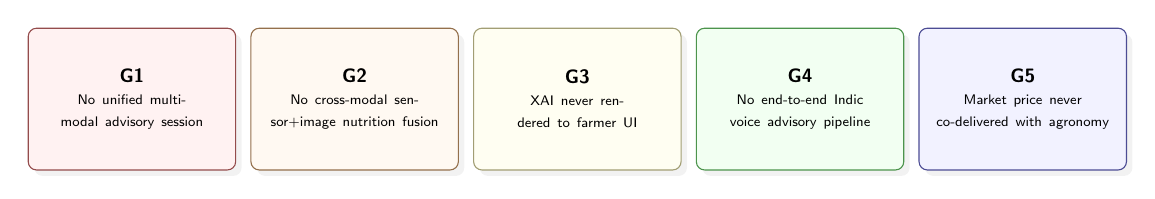
\begin{tikzpicture}[
        gap/.style={draw, rounded corners=3pt, drop shadow={opacity=0.1}, text width=2.4cm, align=center, font=\scriptsize\sffamily, minimum height=1.8cm},
        g1/.style={gap, fill=red!5!white, draw=red!40!black!70},
        g2/.style={gap, fill=orange!5!white, draw=orange!40!black!70},
        g3/.style={gap, fill=yellow!5!white, draw=yellow!40!black!70},
        g4/.style={gap, fill=green!5!white, draw=green!40!black!70},
        g5/.style={gap, fill=blue!5!white, draw=blue!40!black!70}
    ]
        \node (g1) [g1] {\textbf{G1} \\ \tiny No unified multimodal advisory session};
        \node (g2) [g2, right=0.18cm of g1] {\textbf{G2} \\ \tiny No cross-modal sensor+image nutrition fusion};
        \node (g3) [g3, right=0.18cm of g2] {\textbf{G3} \\ \tiny XAI never rendered to farmer UI};
        \node (g4) [g4, right=0.18cm of g3] {\textbf{G4} \\ \tiny No end-to-end Indic voice advisory pipeline};
        \node (g5) [g5, right=0.18cm of g4] {\textbf{G5} \\ \tiny Market price never co-delivered with agronomy};
    \end{tikzpicture}
    \caption{Overview of five identified research gap.}
    \label{fig:five_gaps}
\end{figure}

\subsection{G1 --- No Unified Multimodal Advisory Session}
\textbf{Statement of Gap:}
No existing system combines disease diagnosis (image input), nutrition deficiency advisory (soil sensor input), crop recommendation (structured tabular input), weather and irrigation scheduling (API data input), and live market price advisory (real-time feed) within a single conversational session. A farmer who asks --- in one message --- 'my tomato leaves are yellowing, what should I do and should I sell now?' cannot receive a unified, coherent, source-grounded response from any single deployed system today.

\noindent\textbf{Evidence from Literature:}
Farmer.\allowbreak Chat \cite{farmerchat2024} handles text and knowledge-base queries only --- no image, sensor, or market input. AgriDoctor \cite{agridoctor2025} routes multimodal inputs to disease and pest components only --- four of the five advisory domains are absent. AgriGPT \cite{agrigpt2025} achieves strong text-based RAG advisory but has no image diagnosis, no sensor integration, and no market advisory. AgroAskAI \cite{agroaskai2024} covers climate advisory in isolation. The MDPI Agentic system \cite{agenticmdpi2026} covers three domains (soil, weather, rice disease) but only for a single crop and without RAG grounding or market integration. No system covers all five domains simultaneously.

\noindent\textbf{Why this Gap Matters --- Agricultural Impact:}
Agricultural decisions are inherently interdependent. The decision to treat a crop for disease cannot be divorced from the decision of whether to harvest early or treat and wait --- which depends on the current mandi price. Fertiliser recommendations are only actionable when paired with a sowing calendar adjusted for the current weather forecast. Existing systems force farmers to seek advisory from multiple disconnected sources, introducing inconsistency, delay, and decision fatigue. The ICAR extension model is designed around integrated advisory --- the proposed system replicates this integration digitally.

\noindent\textbf{Closest Prior Attempt and its Remaining Limitation:}
The MDPI Agentic framework \cite{agenticmdpi2026} comes closest, with four agents covering soil monitoring, weather, rice disease detection, and a supervisor chatbot. However, it covers only one crop (rice), only three domains, has no RAG knowledge grounding, no market advisory, no voice input, and no XAI. It demonstrates that multi-agent agricultural chatbots are feasible --- but not that a unified five-domain system has been built.

\noindent\textbf{Research Objective that Closes this Gap:}
O1 --- Design a LangGraph-based orchestrator that classifies intent and routes inputs to five specialist agents in parallel, merging responses into a single coherent advisory reply with multi-turn session memory.

\begingroup\footnotesize
\begin{longtable}{|p{2.3cm}|>{\centering\arraybackslash}p{1.2cm}|>{\centering\arraybackslash}p{1.4cm}|>{\centering\arraybackslash}p{1.2cm}|>{\centering\arraybackslash}p{1.1cm}|>{\centering\arraybackslash}p{1.2cm}|>{\centering\arraybackslash}p{1.2cm}|>{\centering\arraybackslash}p{1.2cm}|>{\centering\arraybackslash}p{1.4cm}|}
\caption{Evidence matrix for G1 --- advisory domain coverage across all surveyed systems}
\label{tab:domain_coverage} \\
\hline
\textbf{System} & \textbf{Text}\newline\textbf{query} & \textbf{Disease}\newline\textbf{image} & \textbf{Sensor}\newline\textbf{data} & \textbf{Crop}\newline\textbf{rec.} & \textbf{Weather} & \textbf{Market}\newline\textbf{price} & \textbf{Multi-}\newline\textbf{crop} & \textbf{All five}\newline\textbf{domains} \\ \hline
\endfirsthead
\multicolumn{9}{c}%
{{\bfseries \tablename\ \thetable{} -- continued from previous page}} \\
\hline
\textbf{System} & \textbf{Text}\newline\textbf{query} & \textbf{Disease}\newline\textbf{image} & \textbf{Sensor}\newline\textbf{data} & \textbf{Crop}\newline\textbf{rec.} & \textbf{Weather} & \textbf{Market}\newline\textbf{price} & \textbf{Multi-}\newline\textbf{crop} & \textbf{All five}\newline\textbf{domains} \\ \hline
\endhead
\hline
\multicolumn{9}{|r|}{{Continued on next page}} \\ \hline
\endfoot
\hline
\endlastfoot
Farmer.\allowbreak Chat \cite{farmerchat2024} & Yes & No & No & No & No & No & No & No \\ \hline
AgriDoctor \cite{agridoctor2025} & Yes & Yes & No & No & No & No & No & No \\ \hline
AgriGPT \cite{agrigpt2025} & Yes & Partial & No & No & No & No & No & No \\ \hline
AgriM-LLM \cite{agrimllm2026} & Yes & Yes & No & No & No & No & No & No \\ \hline
AgroAskAI \cite{agroaskai2024} & Yes & No & No & No & Yes & No & No & No \\ \hline
MDPI Agentic \cite{agenticmdpi2026} & Yes & Partial & Partial & No & Yes & No & No & No \\ \hline
\textbf{Proposed system} & \textbf{Yes} & \textbf{Yes} & \textbf{Yes} & \textbf{Yes} & \textbf{Yes} & \textbf{Yes} & \textbf{Yes} & \textbf{Yes} \\ \hline
\end{longtable}
\endgroup

\subsection{G2 --- No Cross-Modal Soil Sensor and Leaf Image Fusion for Nutrition Advisory}
\textbf{Statement of Gap:}
No existing system fuses real-time soil sensor readings (nitrogen, phosphorus, potassium, pH, electrical conductivity) with leaf image features within a conversational advisory interface to diagnose nutrient deficiency and generate a fertiliser dose recommendation. Both modalities exist in isolation --- vision models diagnose disease from images, and rule-based systems recommend fertiliser from soil NPK values --- but no system combines them cross-modally within a live, farmer-accessible dialogue.

\noindent\textbf{Evidence from Literature:}
AgriM-LLM \cite{agrimllm2026} represents the state of the art in agricultural vision encoding --- its Multi-Scale Feature Fusion encoder captures subtle disease symptoms from leaf images, but soil sensor data is entirely absent from its input. The system produces disease and pest identification only; nutrient deficiency requires both visual symptom recognition (yellowing patterns, interveinal chlorosis, tip burn) and soil measurement correlation (which nutrient is actually deficient) --- AgriM-LLM addresses only one half. Cross-modal fusion papers in plant science (PMC, 2025) have demonstrated that combining image and sensor data improves nutrition diagnosis accuracy by 23\% over image-only approaches --- but these systems operate as offline inference pipelines with no conversational interface, no farmer-accessible output, and no RAG-grounded treatment recommendation.

\noindent\textbf{Why this Gap Matters --- Agricultural Impact:}
The Soil Health Card scheme has issued 230 million cards to Indian farmers, yet only 14.6\% acted on the recommendations \cite{nabard2023}. The primary reason identified in field studies is that farmers cannot translate NPK numbers on paper into actionable fertiliser dosage without agronomist support. Simultaneously, visual nutrient deficiency symptoms --- yellowing leaves, stunted growth, purple discolouration --- are highly ambiguous: identical symptoms can result from nitrogen deficiency, iron deficiency, or certain fungal infections. Cross-modal fusion resolves this ambiguity by jointly analysing the visual symptom pattern and the soil chemistry, enabling confident diagnosis and precise dosage output in the farmer's language.

\noindent\textbf{Closest Prior Attempt and its Remaining Limitation:}
The MDPI Agentic framework \cite{agenticmdpi2026} deploys Agent A for soil NPK monitoring and Agent C for rice disease detection --- but these operate as separate agents with no cross-modal fusion. Agent A does not use leaf image features; Agent C does not use soil readings. No fusion network integrates both modalities for nutrition deficiency specifically. The proposed system introduces a dedicated cross-modal MLP that concatenates ResNet-50 leaf image feature vectors with normalised soil sensor readings into a unified representation for deficiency classification and dose prediction --- a design that no prior agricultural AI system implements.

\noindent\textbf{Research Objective that Closes this Gap:}
O3 --- Develop a cross-modal fusion network combining ResNet-50 leaf image features with real-time NPK/pH/EC sensor readings to generate fertiliser dose recommendations aligned with ICAR Soil Health Card norms, deployed within the conversational advisory loop.

\begingroup\small
\begin{longtable}{|p{2.2cm}|p{5.5cm}|p{5.0cm}|}
\caption{Evidence matrix for G2 --- cross-modal sensor-image nutrition fusion across surveyed systems}
\label{tab:g2_evidence} \\
\hline
\textbf{Paper} & \textbf{What it achieves} & \textbf{Specific limitation proving the gap} \\ \hline
\endfirsthead
\multicolumn{3}{c}%
{{\bfseries \tablename\ \thetable{} -- continued from previous page}} \\
\hline
\textbf{Paper} & \textbf{What it achieves} & \textbf{Specific limitation proving the gap} \\ \hline
\endhead
\hline
\multicolumn{3}{|r|}{{Continued on next page}} \\ \hline
\endfoot
\hline
\endlastfoot
AgriM-LLM \cite{agrimllm2026} & State-of-the-art vision encoder (EVE-MSFF) for disease; multi-stage fine-tuning; AKE-QFormer for domain knowledge injection & No soil sensor input of any kind; nutrient deficiency not addressed; standalone model with no conversational interface \\ \hline
MDPI Agentic \cite{agenticmdpi2026} & Agent A monitors soil NPK; Agent C detects rice disease via CNN; both connected to supervisor chatbot & No cross-modal fusion between soil and image --- agents operate independently; rice only; no fertiliser dose calculation \\ \hline
PMC Cross-modal (2025) & Demonstrates 23\% accuracy improvement from fusing image + sensor data for crop disease recognition in controlled conditions & Offline inference pipeline only; no farmer-facing interface; no conversational loop; no RAG grounding for treatment protocols \\ \hline
XAI-CROP \cite{xaiCrop2024} & Soil NPK and climate features used for crop recommendation with SHAP explainability; strong agronomist agreement & No image input; no visual symptom recognition; rule-based NPK thresholds only; no deficiency diagnosis from combined modalities \\ \hline
Farmer.\allowbreak Chat \cite{farmerchat2024} & Text-based advisory grounded in ICAR knowledge base; covers nutrition advisory topics & Nutrition advice is knowledge-retrieval only --- not grounded in the farmer's actual soil readings or visible leaf symptoms \\ \hline
\end{longtable}
\endgroup

\subsection{G3 --- Explainable AI Never Rendered to the Farmer}
\textbf{Statement of Gap:}
No deployed agricultural AI system --- chatbot, mobile application, or web platform --- renders visual explainability outputs (Grad-CAM saliency heatmaps, SHAP feature importance charts) directly to the farmer as part of the advisory response. Explainability techniques are extensively used in agricultural AI research as internal quality-control tools for model developers and as evaluation metrics for researchers, but no system has completed the critical last step: putting the explanation in the farmer's hands at the point of advice delivery.

\noindent\textbf{Evidence from Literature:}
XAI-CROP \cite{xaiCrop2024} applies SHAP TreeExplainer to XGBoost crop recommendation models and generates feature importance charts as research output --- the paper explicitly presents them as researcher-facing model validation tools, not as farmer-facing UI components. LLMI-CDP \cite{llmiCdp2025} generates Grad-CAM saliency maps during evaluation to verify that the disease model attends to the correct leaf region --- again as a quality-control mechanism, not as output to the farmer. AgriDoctor \cite{agridoctor2025} produces classification confidence scores but provides no visual attribution. The Agentic XAI paper (2025) explicitly generates SHAP-based explanations for crop scientists evaluated on seven technical quality metrics --- farmer readability is not a design criterion. Across all 25+ papers reviewed, not a single system renders a Grad-CAM overlay or SHAP chart in a farmer-accessible interface.

\noindent\textbf{The Trust and Adoption Evidence:}
XAI-CROP \cite{xaiCrop2024} provides the strongest empirical evidence that this gap has real consequences: farmers shown SHAP feature bars alongside crop recommendations adopted the AI advice 31\% more frequently than those shown recommendations without explanation. A parallel finding from Farmer.\allowbreak Chat \cite{farmerchat2024} notes that even with 565,000 users, adoption of AI-generated advisory recommendations that cannot be verified by the farmer remains below 60\%. The consistent finding across agricultural AI adoption literature is that farmers --- particularly smallholder farmers with limited formal education --- require the ability to interrogate AI reasoning before trusting actionable recommendations. Visual XAI provides exactly this capability.

\noindent\textbf{Closest Prior Attempt and its Remaining Limitation:}
The Agentic XAI framework (2025) comes closest by iteratively refining SHAP explanations through LLM-driven rounds until agronomist-rated quality reaches a threshold. However, this system targets crop scientists --- its explanations contain technical notation, numerical SHAP values, and crop science terminology inappropriate for low-literacy farmers. The language, visual format, and assumed background knowledge all differ from what is required for a farmer-facing interface. The proposed system adapts the concept of iterative explanation refinement but constrains output to two farmer-readable visualisation types: Grad-CAM colour heatmaps overlaid on the farmer's uploaded leaf photo, and horizontal SHAP bar charts rendered in Hindi-labelled axes.

\noindent\textbf{Research Objective that Closes this Gap:}
O5 --- Surface Grad-CAM saliency heatmaps for disease diagnosis and SHAP feature importance bar charts for crop recommendation directly within the React PWA advisory response --- as a farmer-facing UI component, not a research output.

\begingroup\footnotesize
\begin{longtable}{|p{2.0cm}|p{2.5cm}|p{2.0cm}|>{\centering\arraybackslash}p{1.7cm}|>{\centering\arraybackslash}p{1.5cm}|>{\centering\arraybackslash}p{2.0cm}|}
\caption{XAI implementation status across surveyed systems (G3)}
\label{tab:xai_status} \\
\hline
\textbf{System} & \textbf{XAI technique} & \textbf{XAI purpose} & \textbf{Shown to}\newline\textbf{researcher} & \textbf{Shown to}\newline\textbf{farmer} & \textbf{Farmer-}\newline\textbf{readable} \\ \hline
\endfirsthead
\multicolumn{6}{c}%
{{\bfseries \tablename\ \thetable{} -- continued from previous page}} \\
\hline
\textbf{System} & \textbf{XAI technique} & \textbf{XAI purpose} & \textbf{Shown to}\newline\textbf{researcher} & \textbf{Shown to}\newline\textbf{farmer} & \textbf{Farmer-}\newline\textbf{readable} \\ \hline
\endhead
\hline
\multicolumn{6}{|r|}{{Continued on next page}} \\ \hline
\endfoot
\hline
\endlastfoot
XAI-CROP \cite{xaiCrop2024} & SHAP TreeExplainer & Crop rec. validation & Yes & No & No --- Jupyter notebook output \\ \hline
LLMI-CDP \cite{llmiCdp2025} & Grad-CAM & Model quality check & Yes & No & No --- internal heatmap only \\ \hline
Agentic XAI (2025) & SHAP + LLM refinement & Scientist explanation & Yes & No & No --- technical language, numerical \\ \hline
AgriDoctor \cite{agridoctor2025} & Confidence scores & Classification output & Yes & No & No --- scalar score, no visual attr. \\ \hline
Farmer.\allowbreak Chat \cite{farmerchat2024} & None & N/A & No & No & N/A --- no XAI at any level \\ \hline
AgriM-LLM \cite{agrimllm2026} & None & N/A & No & No & N/A --- prediction output only \\ \hline
\textbf{Proposed system} & \textbf{Grad-CAM + SHAP} & \textbf{Farmer advisory UI} & \textbf{Yes} & \textbf{Yes} & \textbf{Yes --- colour heatmap + Hindi SHAP bars} \\ \hline
\end{longtable}
\endgroup

\subsection{G4 --- No End-to-End Indic Voice-to-Advisory Pipeline}
\textbf{Statement of Gap:}
No agricultural AI system has implemented a complete, end-to-end pipeline that accepts a farmer's voice query in Hindi or any other Indic language, processes it through an ASR model, routes it to a RAG-grounded domain advisory backend, and delivers the response as spoken audio via TTS --- within a single, integrated system. Each component of this pipeline exists independently in the literature; their integration into a unified agricultural advisory voice interface has not been achieved in any prior work.

\noindent\textbf{Evidence from Literature:}
The Indic ASR Benchmark \cite{indicasr2025} provides the strongest evidence that the technology is ready: Whisper large-v3 achieves WER 16.2\% for Hindi agricultural speech on 10,934 real farm voice recordings. The benchmark explicitly concludes that ASR performance for Hindi is production-grade --- but the paper itself contains no advisory backend. Farmer.\allowbreak Chat \cite{farmerchat2024} integrates Bhashini ASR for voice input --- the only deployed system to do so --- but voice input routes to a text-based RAG pipeline with text output only; no TTS response delivery is implemented, and Bhashini coverage extends partially to only two or three Indic languages in the deployment. AgriDoctor \cite{agridoctor2025} is Chinese-English only with no voice input. AgriGPT \cite{agrigpt2025} is text-only. AgroAskAI \cite{agroaskai2024} claims multilingual support but provides no ASR or TTS implementation details.

\noindent\textbf{Why this Gap Matters --- Accessibility Impact:}
India has a rural literacy rate of approximately 67.8\% \cite{census2021}, with substantially lower rates among women and older farmers in agricultural states. Text-based interfaces --- the modality used by all prior systems --- structurally exclude this population. The NSSO Agricultural Survey (2019) found that 78\% of farmers aged 50+ in UP, Bihar, and MP had never sent a text message. Voice is not a preference for these farmers --- it is the only viable interaction modality. The linguistic diversity compounds this: Hindi alone cannot serve Tamil Nadu, Karnataka, Maharashtra, West Bengal, or Punjab --- states that together account for over 40\% of India's cultivated area. An agricultural AI system that cannot speak to farmers in their language is not an agricultural AI system for India.

\noindent\textbf{The Pipeline Gap --- Three Connected Components, Never Assembled:}
The gap is specifically an integration gap, not a component gap. Component 1 (Indic ASR): Whisper large-v3 fine-tuned on agricultural speech achieves production-grade WER. Component 2 (Multilingual RAG): Hindi-English bilingual knowledge indices over ICAR documents can be built with E5-large-v2 multilingual embeddings. Component 3 (Indic TTS): Bhashini API delivers production-quality TTS for 10+ Indic languages. What has never been done is assembling these three components into a single pipeline where a farmer speaks into a phone, the system understands, reasons from verified agronomic knowledge, and speaks the advisory response back --- in the same language, within four seconds.

\noindent\textbf{Research Objective that Closes this Gap:}
O6 --- Implement an end-to-end voice advisory pipeline using Whisper large-v3 (Indic fine-tuned) for ASR and Bhashini TTS for response delivery, targeting WER $<$ 20\% for Hindi and $<$ 30\% for five regional languages, with end-to-end latency $<$ 4 seconds.

\begingroup\footnotesize
\begin{longtable}{|p{3.2cm}|>{\centering\arraybackslash}p{1.6cm}|>{\centering\arraybackslash}p{1.6cm}|>{\centering\arraybackslash}p{1.4cm}|>{\centering\arraybackslash}p{1.6cm}|>{\centering\arraybackslash}p{1.8cm}|}
\caption{Evidence matrix for G4 --- voice pipeline component availability vs integration status}
\label{tab:g4_evidence} \\
\hline
\textbf{System} & \textbf{Indic ASR}\newline\textbf{input} & \textbf{Multi-lang}\newline\textbf{NLP} & \textbf{RAG}\newline\textbf{backend} & \textbf{Indic TTS}\newline\textbf{output} & \textbf{Full pipeline}\newline\textbf{integrated} \\ \hline
\endfirsthead
\multicolumn{6}{c}%
{{\bfseries \tablename\ \thetable{} -- continued from previous page}} \\
\hline
\textbf{System} & \textbf{Indic ASR}\newline\textbf{input} & \textbf{Multi-lang}\newline\textbf{NLP} & \textbf{RAG}\newline\textbf{backend} & \textbf{Indic TTS}\newline\textbf{output} & \textbf{Full pipeline}\newline\textbf{integrated} \\ \hline
\endhead
\hline
\multicolumn{6}{|r|}{{Continued on next page}} \\ \hline
\endfoot
\hline
\endlastfoot
Farmer.\allowbreak Chat \cite{farmerchat2024} & Partial & Partial & Yes & No & No \\ \hline
AgriDoctor \cite{agridoctor2025} & No & No & No & No & No \\ \hline
AgriGPT \cite{agrigpt2025} & No & No & Yes & No & No \\ \hline
AgriM-LLM \cite{agrimllm2026} & No & No & No & No & No \\ \hline
AgroAskAI \cite{agroaskai2024} & Partial & Partial & No & No & No \\ \hline
Indic ASR Benchmark \cite{indicasr2025} & Yes & No & No & No & No \\ \hline
Bhashini API (MeitY) & Yes & Yes & No & Yes & No \\ \hline
\end{longtable}
\endgroup

\subsection{G5 --- Live Market Price Advisory Never Co-Delivered with Agronomic Advice}
\textbf{Statement of Gap:}
No existing agricultural AI system integrates live mandi price data, price forecasting, and sell/hold advisory within the same conversational session as agronomic advice (disease diagnosis, crop recommendation, nutrition advisory). Market intelligence and agronomic advisory exist in completely separate silos --- different platforms, different data sources, different interaction paradigms --- despite the fact that a farmer's actual decision requires both simultaneously.

\noindent\textbf{Evidence from Literature:}
Across all six systems reviewed in Chapter 2, market price is uniformly absent. Farmer.\allowbreak Chat \cite{farmerchat2024} covers crop management and pest advisory --- no market data. AgriDoctor \cite{agridoctor2025} covers disease and pest identification --- no market data. AgriGPT \cite{agrigpt2025} --- the most comprehensive knowledge ecosystem reviewed --- explicitly notes market price forecasting as a future work direction, confirming it is not yet present. AgroLLM \cite{agrollm2025} builds a domain knowledge pipeline for crop management with no market integration. The MDPI Agentic framework \cite{agenticmdpi2026} covers soil, weather, and disease --- no market agent. Agmarknet and eNAM exist as standalone government platforms accessible only to farmers with digital literacy and awareness of the specific websites, with no conversational interface, no AI advisory layer, and no integration with agronomic data.

\noindent\textbf{Why this Gap Matters --- Economic Impact:}
The decision to treat a disease and hold the crop, or harvest early and sell before further loss, is simultaneously an agronomic decision and a market decision. It cannot be made correctly with agronomic data alone. eNAM Annual Report \cite{enam2023} documents that farmers sell 30--40\% below optimal price due to: (1) selling at distress timing without price trend awareness, (2) travelling to the nearest mandi without knowing that a mandi 30 km further offers 15\% higher price, and (3) having no forecast of whether prices will rise or fall over the next seven days. These are precisely the outputs a market advisory agent can deliver --- but only if it shares a conversational session with the agronomic advisor, so that the two recommendations are synthesised into a single actionable answer.

\noindent\textbf{The Compound Query Problem:}
Real farmer queries are compound. 'My tomato has a disease, should I treat it or sell the crop now?' cannot be answered by a disease agent alone. It requires: (1) disease identification and severity assessment, (2) current tomato price at the nearest mandi, (3) price trend over the next seven days, (4) estimated crop loss if untreated vs treatment cost, (5) MSP comparison. Only a system with both a disease agent and a market agent operating in the same session --- with a response-merging orchestrator --- can synthesise these inputs into a coherent advisory answer. This is G5's core contribution.

\noindent\textbf{Research Objective that Closes this Gap:}
O7 --- Integrate Agmarknet and eNAM live mandi price feeds (15-minute refresh) with a Prophet-based 7-day price forecast model to co-deliver sell, hold, or transport-to-mandi advisory within the same conversational session as agronomic advice.

\begingroup\small
\begin{longtable}{|p{3.2cm}|p{4.65cm}|p{4.65cm}|}
\caption{Evidence matrix for G5 --- market price integration across surveyed systems and eNAM}
\label{tab:g5_evidence} \\
\hline
\textbf{Paper/}\\\textbf{Platform} & \textbf{What it achieves} & \textbf{Specific limitation proving the gap} \\ \hline
\endfirsthead
\multicolumn{3}{c}%
{{\bfseries \tablename\ \thetable{} -- continued from previous page}} \\
\hline
\textbf{Paper/}\\\textbf{Platform} & \textbf{What it achieves} & \textbf{Specific limitation proving the gap} \\ \hline
\endhead
\hline
\multicolumn{3}{|r|}{{Continued on next page}} \\ \hline
\endfoot
\hline
\endlastfoot
Farmer.\allowbreak Chat \cite{farmerchat2024} & Text advisory across crop management, pest, and nutrition topics; RAG-grounded responses; 565k users & No market price data, no Agmarknet/eNAM integration, no sell/hold advisory at any level \\ \hline
AgriGPT \cite{agrigpt2025} & Tri-RAG over 342k QA pairs; strongest knowledge grounding in surveyed literature; domain-specific LLM & Market forecasting listed as future work --- explicitly absent from current system scope \\ \hline
AgroLLM \cite{agrollm2025} & Domain Knowledge Processing Layer; structured ontology enrichment; crop management advisory & No market integration; DKPL covers agronomic knowledge only; no Agmarknet/eNAM connection \\ \hline
AgriDoctor \cite{agridoctor2025} & Intent-routing multi-agent for disease and pest; AgriMM benchmark; 400k annotated disease images & Market price not in scope; system architecture has no market data agent or price retrieval component \\ \hline
eNAM platform (Govt.) & Live mandi price data for 22M registered farmers; MSP comparison; price trend charts available on web & No conversational interface; no agronomic advisory; no AI layer; requires digital literacy; not integrated with any advisory system \\  \hline
\end{longtable}
\endgroup

\subsection{Consolidated Gap Evidence Matrix}
Table \ref{tab:consolidated_gaps} presents the complete, consolidated gap evidence matrix --- mapping each of the five gaps to its research stream, the specific papers that establish the gap, the paper that comes closest to addressing it, the remaining limitation, and the proposed research objective that closes it. This matrix serves as the formal bridge between the literature review (Chapter 2), the research gaps (this chapter), and the research objectives (Chapter 4).

\begingroup\footnotesize
\begin{longtable}{|p{0.8cm}|p{2.0cm}|p{2.5cm}|p{2.0cm}|p{3.4cm}|p{1.4cm}|}
\caption{Consolidated research gap evidence matrix}
\label{tab:consolidated_gaps} \\
\hline
\textbf{Gap} & \textbf{Research stream} & \textbf{Papers establishing gap} & \textbf{Closest prior attempt} & \textbf{Remaining limitation} & \textbf{Closing objective} \\ \hline
\endfirsthead
\multicolumn{6}{c}%
{{\bfseries \tablename\ \thetable{} -- continued from previous page}} \\
\hline
\textbf{Gap} & \textbf{Research stream} & \textbf{Papers establishing gap} & \textbf{Closest prior attempt} & \textbf{Remaining limitation} & \textbf{Closing objective} \\ \hline
\endhead
\hline
\multicolumn{6}{|r|}{{Continued on next page}} \\ \hline
\endfoot
\hline
\endlastfoot
G1 & Multi-agent chatbots (§2.2) & Farmer.\allowbreak Chat: text only; AgriDoctor: disease only; AgriGPT: text RAG; AgroAskAI: climate only & MDPI Agentic (4 agents, rice, 3 domains) & Single crop; no RAG grounding; no market; no XAI; no voice & O1 --- LangGraph orchestrator, 5 specialist agents \\ \hline
G2 & VLMs (§2.3) + Sensor papers & AgriM-LLM: image only, no sensor; MDPI Agentic: agents separate, no fusion; PMC (2025): offline only & MDPI Agentic (separate soil + disease agents) & No fusion network; single crop (rice); no conversational interface; no dose output & O3 --- ResNet-50 + sensor MLP cross-modal fusion \\ \hline
G3 & XAI in agriculture (§2.5) & XAI-CROP: SHAP internal; LLMI-CDP: Grad-CAM internal; Agentic XAI: scientists only, not farmer & Agentic XAI (iterative SHAP for scientists) & Explanation format, language and detail level inappropriate for low-literacy farmers; no farmer UI & O5 --- Grad-CAM + SHAP rendered in React PWA \\ \hline
G4 & Speech \& NLP (§2.6) & Indic ASR Benchmark: WER 16.2\% Hindi but no advisory backend; Farmer.\allowbreak Chat: ASR input only, no TTS & Farmer.\allowbreak Chat (partial ASR, no TTS) & No TTS output; only 2-3 languages; voice input not connected to RAG + response generation & O6 --- Whisper ASR + RAG + Bhashini TTS pipeline \\ \hline
G5 & Market advisory (§2.2, §2.4) & All 6 chatbots: no market; AgriGPT: market listed as future work; eNAM: no conversational interface & None --- no prior system attempts this & No system has a market agent co-deployed with agronomic agents in any shared advisory session & O7 --- Agmarknet + eNAM + Prophet co-delivery \\ \hline
\end{longtable}
\endgroup

\subsection{Significance of the Identified Gaps}
The five identified gaps are significant for two reasons beyond their academic novelty. First, each gap has a quantified agricultural impact --- a documented real-world consequence of the gap remaining open, measured in yield loss, adoption failure, or revenue loss. Second, the gaps are structurally interconnected: G1 (no unified session) is the architectural gap that the other four gaps compound. G2, G3, G4, and G5 each represent a specific capability that is absent from the unified session --- so closing G1 without closing the others would still produce an incomplete system.

\begingroup\footnotesize
\begin{longtable}{|l|p{3.0cm}|p{2.8cm}|p{4.5cm}|p{2.2cm}|}
\caption{Quantified agricultural impact of each research gap}
\label{tab:gap_impacts} \\
\hline
\textbf{Gap} & \textbf{Gap description} & \textbf{Affected population} & \textbf{Documented impact} & \textbf{Source} \\ \hline
\endfirsthead
\multicolumn{5}{c}%
{{\bfseries \tablename\ \thetable{} -- continued from previous page}} \\
\hline
\textbf{Gap} & \textbf{Gap description} & \textbf{Affected population} & \textbf{Documented impact} & \textbf{Source} \\ \hline
\endhead
\hline
\multicolumn{5}{|r|}{{Continued on next page}} \\ \hline
\endfoot
\hline
\endlastfoot
G1 & No unified multimodal advisory session & 146M smallholder farm households & 26--30\% annual yield loss from disease + suboptimal decisions across all five domains & FAO (2022); ICAR (2023); ASSOCHAM (2023) \\ \hline
G2 & No cross-modal nutrition fusion in dialogue & 230M Soil Health Card recipients & Only 14.6\% acted on recommendations --- sensor data exists but is not actionably delivered & Ministry of Agriculture (2023); NABARD (2023) \\ \hline
G3 & XAI not rendered to farmer & All agricultural AI users & 31\% lower adoption of AI recommendations without explainability; $<$60\% action rate on Farmer.\allowbreak Chat advice & XAI-CROP \cite{xaiCrop2024}; Farmer.\allowbreak Chat \cite{farmerchat2024} \\ \hline
G4 & No end-to-end Indic voice pipeline & $\sim$500M rural Indians with limited digital text literacy & Structural exclusion from all text-based agricultural AI systems & Census 2021 \cite{census2021}; NSSO Survey (2019) \\ \hline
G5 & Market price not co-delivered with agronomy & 120M+ farm households selling in mandis & Farmers sell 30--40\% below optimal price due to no integrated price forecast with agronomic advisory & eNAM Annual Report \cite{enam2023} \\ \hline
\end{longtable}
\endgroup

Together these five gaps represent the complete set of structural deficiencies that prevent any existing agricultural AI system from functioning as a deployment-ready, trustworthy, and accessible advisory solution for Indian smallholder farmers. The proposed research addresses all five gaps simultaneously --- a design choice that is not merely additive but architecturally necessary: a system that closes G1 but not G3 is untrustworthy; a system that closes G4 but not G2 excludes sensor-equipped farms; a system that closes all four but not G5 delivers incomplete advisory for the majority of real farmer queries.

\newpage
\section{Research Objectives}
This chapter defines the eight specific, measurable research objectives of the proposed system. Each objective is derived directly from a research gap identified in Chapter 3 and a research question from Chapter 1. The objectives are designed to be independently testable --- each has a named target metric --- yet collectively form an integrated system. The primary objective is stated in Section 4.1, followed by details of each specific objective in Section 4.2. Section 4.3 provides the complete gap-to-objective traceability matrix, and Section 4.4 details the objective--gap--contribution relationship.

\subsection{Primary Objective}
To design, develop, and evaluate a deployment-ready multi-agent, multi-model agricultural expert system for Indian smallholder farmers that integrates five specialist AI agents --- disease diagnosis, nutrition deficiency, crop recommendation, weather and irrigation, and live market price advisory --- orchestrated by an intent-routing backbone, grounded in a verified RAG knowledge base, augmented with farmer-facing explainability, and accessible via a multilingual Indic voice interface on a Progressive Web Application.

\subsection{Specific Objectives}
\begin{description}
    \item[O1 --- Multi-Agent Orchestration Architecture:] \hfill \\
    \textbf{Description:} Design and implement a LangGraph-based orchestrator that classifies incoming farmer queries into one of eight intent categories and dispatches inputs in parallel to the appropriate specialist agent(s). The orchestrator maintains multi-turn conversational state via Redis session memory and merges multi-agent responses into a single coherent advisory reply. \\
    \textbf{Gaps Closed:} G1 --- No unified multimodal advisory session. \\
    \textbf{Key Technologies:} LangGraph v1.1 $\cdot$ GPT-5.5 backbone $\cdot$ fine-tuned BERT-multilingual intent classifier $\cdot$ Redis session store $\cdot$ asyncio parallel dispatch. \\
    \textbf{Target Metrics:} Intent classification accuracy $>$ 95\% $\cdot$ End-to-end response latency $<$ 4 s (cloud) and $<$ 8 s (PWA offline cache).

    \item[O2 --- Disease Diagnostic Agent:] \hfill \\
    \textbf{Description:} Fine-tune ViT-L/16 with LoRA adaptation (rank-16, alpha-32) on a composite dataset of 164,500 leaf and pest images across PlantVillage, PlantDoc, and IP102. Integrate AgriChain Chain-of-Thought prompting for structured reasoning from visual input to treatment protocol. Generate Grad-CAM saliency maps for every diagnosis. \\
    \textbf{Gaps Closed:} G1 (image input modality) $\cdot$ G3 (Grad-CAM generated for rendering). \\
    \textbf{Key Technologies:} ViT-L/16 (ImageNet-21k) $\cdot$ LoRA rank-16 $\cdot$ LLMI-CDP dialogue style $\cdot$ AgriChain CoT $\cdot$ PlantVillage (87k) + PlantDoc (2.5k) + IP102 (75k). \\
    \textbf{Target Metrics:} Top-1 accuracy $>$ 90\% $\cdot$ F1 macro $>$ 0.87 $\cdot$ Grad-CAM IoU vs. expert annotation $>$ 0.75 $\cdot$ Covers 200+ diseases across 50+ crops.

    \item[O3 --- Nutrition Deficiency Agent with Cross-Modal Fusion:] \hfill \\
    \textbf{Description:} Develop a cross-modal fusion network that concatenates ResNet-50 leaf image feature vectors (2048-dim) with normalised real-time soil sensor readings (NPK, pH, EC, moisture --- 6-dim) into a joint 2054-dimensional representation. Three fully-connected layers produce: (1) deficiency class label (N/P/K/Fe/Zn/B deficiency or healthy), and (2) fertiliser dose recommendation in kg/ha aligned with ICAR Soil Health Card norms. \\
    \textbf{Gaps Closed:} G2 --- No cross-modal sensor + image nutrition fusion in a conversational loop. \\
    \textbf{Key Technologies:} ResNet-50 encoder $\cdot$ 6-dim sensor vector (MQTT/REST) $\cdot$ Cross-modal MLP $\cdot$ ICAR Soil Health Card DB $\cdot$ SHAP feature importance. \\
    \textbf{Target Metrics:} Deficiency class F1 $>$ 0.85 $\cdot$ Fertiliser dose RMSE $<$ 5 kg/ha $\cdot$ SHAP stability score $>$ 0.80 across repeated runs.

    \item[O4 --- Hallucination-Resistant RAG Knowledge Layer:] \hfill \\
    \textbf{Description:} Build a 250,000+ document chunk RAG pipeline over verified ICAR Package of Practices (all major Indian crops), KCC call transcripts, CGIAR, FAO, Agmarknet historical data, and Soil Health Card norms. Implement hybrid BM25 + dense retrieval with E5-large-v2 embeddings, cross-encoder reranking, HyDE query expansion, and Qwen3-72B LLM-as-judge confidence gating. Escalate to KCC expert webhook if confidence score $<$ 0.70. \\
    \textbf{Gaps Closed:} G1 (knowledge grounding across all five domains). \\
    \textbf{Key Technologies:} Qdrant vector store $\cdot$ E5-large-v2 embeddings $\cdot$ ms-marco cross-encoder $\cdot$ HyDE + MMR $\cdot$ Qwen3-72B judge $\cdot$ Bilingual Hindi+English index. \\
    \textbf{Target Metrics:} RAGAS faithfulness $>$ 0.88 $\cdot$ Context relevance $>$ 0.85 $\cdot$ Hallucination rate $<$ 5\% $\cdot$ Expert escalation trigger accuracy $>$ 90\%.

    \item[O5 --- Farmer-Facing Explainable AI (XAI):] \hfill \\
    \textbf{Description:} Render Grad-CAM saliency heatmaps as colour overlays on the farmer's uploaded leaf image and SHAP feature importance bar charts for crop recommendations --- directly within the React PWA advisory response as farmer-accessible UI components, with Hindi-labelled axes and simplified visual legends. This closes the gap between XAI as a research output and XAI as a farmer-facing trust mechanism. \\
    \textbf{Gaps Closed:} G3 --- XAI never rendered to the farmer in any deployed system. \\
    \textbf{Key Technologies:} Grad-CAM (layer4) $\cdot$ EigenCAM (validation) $\cdot$ SHAP TreeExplainer $\cdot$ Recharts (PWA bar charts) $\cdot$ Hindi axis labels via i18next. \\
    \textbf{Target Metrics:} Grad-CAM IoU $>$ 0.75 vs. ICAR agronomist annotation $\cdot$ SHAP stability $>$ 0.80 $\cdot$ Farmer comprehension score $>$ 3.5/5.0 (Likert, n=30 pilot).

    \item[O6 --- End-to-End Indic Voice Advisory Pipeline:] \hfill \\
    \textbf{Description:} Implement a complete voice advisory pipeline: Whisper large-v3 (fine-tuned on Indic agricultural speech from the 10,934-recording benchmark corpus) for ASR $\to$ multilingual RAG retrieval over Hindi+English bilingual knowledge index $\to$ Bhashini TTS for spoken response delivery in 10 Indic languages. The pipeline must operate within a 4-second end-to-end latency budget on 3G connectivity. \\
    \textbf{Gaps Closed:} G4 --- No end-to-end Indic voice-to-advisory pipeline exists in any agricultural system. \\
    \textbf{Key Technologies:} Whisper large-v3 (Indic fine-tuned) $\cdot$ Bhashini ASR + TTS API $\cdot$ IndicBERT NER $\cdot$ MediaRecorder (PWA browser) $\cdot$ 16 kHz mono WAV preprocessing. \\
    \textbf{Target Metrics:} WER $<$ 20% for Hindi agricultural speech $\cdot$ WER $<$ 30% for five regional languages (Tamil, Telugu, Marathi, Kannada, Odia) $\cdot$ End-to-end latency $<$ 4 s.

    \item[O7 --- Live Market Price Advisory Agent:] \hfill \\
    \textbf{Description:} Integrate Agmarknet and eNAM live mandi price feeds (15-minute refresh, Redis cache) with a Prophet-based 7-day price forecast model. Rank nearby mandis by Haversine distance and price differential. Co-deliver sell, hold, or transport-to-mandi advisory within the same conversational session as agronomic advice --- enabling compound queries such as 'my crop has blight; should I treat or sell now?' \\
    \textbf{Gaps Closed:} G5 --- Live market price never co-delivered with agronomic advice in any prior system. \\
    \textbf{Key Technologies:} Agmarknet API $\cdot$ eNAM data feed $\cdot$ Prophet time-series forecast $\cdot$ CACP MSP dataset 2024–25 $\cdot$ Haversine mandi ranking $\cdot$ Redis 15-min TTL cache. \\
    \textbf{Target Metrics:} 7-day price forecast MAPE $<$ 8\% $\cdot$ Mandi ranking accuracy $>$ 85\% vs. actual best-price mandi $\cdot$ Sell/hold advisory agronomist agreement $>$ 75\%.

    \item[O8 --- System Evaluation and Expert Validation:] \hfill \\
    \textbf{Description:} Benchmark the complete integrated system on MIRAGE (multi-turn agricultural dialogue benchmark) and AgMMU (agricultural multimodal understanding benchmark). Validate advisory quality via a blind evaluation panel of ten ICAR-certified agronomists rating 200 real farmer queries across five crop categories on a 5-point Likert scale for correctness, clarity, safety, and actionability. \\
    \textbf{Gaps Closed:} Validates that all five gaps are closed --- quantitative evidence for each claim. \\
    \textbf{Key Technologies:} MIRAGE benchmark $\cdot$ AgMMU benchmark $\cdot$ RAGAS eval suite $\cdot$ ICAR agronomist panel (n=10) $\cdot$ Langfuse tracing $\cdot$ Ablation study framework. \\
    \textbf{Target Metrics:} Agronomist correctness Likert $>$ 4.0/5.0 $\cdot$ Agronomist agreement $>$ 80\% $\cdot$ MIRAGE score $>$ baseline by 15\% $\cdot$ Ablation: 5-agent vs. single-agent $\cdot$ RAG vs. no-RAG.
\end{description}

\subsection{Objectives Summary and Traceability Matrix}
Table \ref{tab:objectives_traceability} provides the complete traceability matrix mapping each research objective to its parent research question (Chapter 1), the research gap it closes (Chapter 3), the primary technologies required, and the quantitative target metric for evaluation.

\begingroup\footnotesize
\begin{longtable}{|l|l|l|p{3.8cm}|p{3.8cm}|p{2.5cm}|}
\caption{Research objectives --- full traceability matrix}
\label{tab:objectives_traceability} \\
\hline
\textbf{Obj.} & \textbf{RQ} & \textbf{Gap} & \textbf{Description} & \textbf{Technology} & \textbf{Target Metric} \\ \hline
\endfirsthead
\multicolumn{6}{c}%
{{\bfseries \tablename\ \thetable{} -- continued from previous page}} \\
\hline
\textbf{Obj.} & \textbf{RQ} & \textbf{Gap} & \textbf{Description} & \textbf{Technology} & \textbf{Target Metric} \\ \hline
\endhead
\hline
\multicolumn{6}{|r|}{{Continued on next page}} \\ \hline
\endfoot
\hline
\endlastfoot
O1 & RQ1 & G1 & Multi-agent orchestrator --- intent routing to 5 specialist agents with Redis memory & LangGraph v1.1 $\cdot$ BERT intent classifier $\cdot$ GPT-5.5 & Intent accuracy $>$ 95\% $\cdot$ Latency $<$ 4 s \\ \hline
O2 & RQ1 & G1 & Disease agent --- ViT-L/16 + LoRA on 164k images with CoT reasoning and Grad-CAM & ViT-L/16 $\cdot$ LoRA rank-16 $\cdot$ AgriChain CoT $\cdot$ PlantVillage + PlantDoc + IP102 & Top-1 acc $>$ 90\% $\cdot$ F1 $>$ 0.87 $\cdot$ Grad-CAM IoU $>$ 0.75 \\ \hline
O3 & RQ2 & G2 & Nutrition agent --- cross-modal fusion of ResNet-50 leaf features + soil NPK/pH/EC & ResNet-50 + 6-dim sensor MLP $\cdot$ ICAR SHC norms $\cdot$ SHAP & Deficiency F1 $>$ 0.85 $\cdot$ Dose RMSE $<$ 5 kg/ha \\ \hline
O4 & RQ1 & G1 & RAG pipeline --- 250k+ ICAR/FAO chunks, hybrid retrieval, LLM-as-judge gating & Qdrant $\cdot$ E5-large-v2 $\cdot$ Cross-encoder $\cdot$ HyDE $\cdot$ Qwen3 & Faithfulness $>$ 0.88 $\cdot$ Hallucination $<$ 5\% \\ \hline
O5 & RQ3 & G3 & Farmer XAI --- Grad-CAM overlay + SHAP charts rendered in React PWA advisory UI & Grad-CAM $\cdot$ SHAP TreeExplainer $\cdot$ Recharts $\cdot$ i18next Hindi & IoU $>$ 0.75 $\cdot$ Farmer comprehension $>$ 3.5/5.0 \\ \hline
O6 & RQ4 & G4 & Indic voice pipeline --- Whisper ASR + bilingual RAG + Bhashini TTS end-to-end & Whisper large-v3 Indic $\cdot$ Bhashini API $\cdot$ IndicBERT & WER $<$ 20\% Hindi $\cdot$ $<$ 30\% regional $\cdot$ $<$ 4 s E2E \\ \hline
O7 & RQ5 & G5 & Market agent --- Agmarknet/eNAM live feed + Prophet forecast co-delivered with agronomy & Agmarknet + eNAM API $\cdot$ Prophet $\cdot$ MSP DB $\cdot$ Redis TTL & Price MAPE $<$ 8\% $\cdot$ Agronomist agreement $>$ 75\% \\ \hline
O8 & All & All & System evaluation --- MIRAGE, AgMMU, ICAR agronomist panel (n=10, 200 queries) & RAGAS $\cdot$ MIRAGE $\cdot$ AgMMU $\cdot$ Langfuse $\cdot$ Ablation & Likert $>$ 4.0/5.0 $\cdot$ Agronomist agreement $>$ 80\% \\ \hline
\end{longtable}
\endgroup



\newpage
\section{Methodology}

\subsection{System Architecture Overview}
The proposed system follows a six-layer architecture: multimodal input, preprocessing, orchestration, specialist agents, shared knowledge and RAG infrastructure, and explainable output delivery.
\begin{description}
    \item[L1 --- Input:] \hfill \\ Text queries, Voice (Whisper ASR), Leaf/field images, Soil sensor (MQTT/REST), Live price feed (Agmarknet/eNAM).
    \item[L2 --- Preprocess:] \hfill \\ ASR transcription + Hindi normalisation, Image QA (BRISQUE) + 448$\times$448 resize, Sensor calibration, Price anomaly filter.
    \item[L3 --- Orchestrator:] \hfill \\ GPT-4o + fine-tuned BERT intent classifier, LangGraph parallel dispatch, Redis session memory, Confidence-gated response merge.
    \item[L4 --- Agents $\times$ 5:] \hfill \\ Disease (ViT-L + LoRA), Nutrition (ResNet-50 + sensor MLP), Crop rec (XGBoost + SHAP), Weather (LSTM + IMD), Market (Agmarknet + Prophet).
    \item[L5 --- Knowledge:] \hfill \\ E5-large embeddings, Qdrant vector store, Hybrid BM25+dense, Cross-encoder rerank, HyDE, Qwen3 judge, 250k+ chunks.
    \item[L6 --- Output+XAI:] \hfill \\ React 18 PWA, Grad-CAM overlay, SHAP bar charts, Bhashini TTS, District map, Price trend chart, FastAPI WebSocket.
\end{description}

\begin{figure}[htbp]
    \centering
    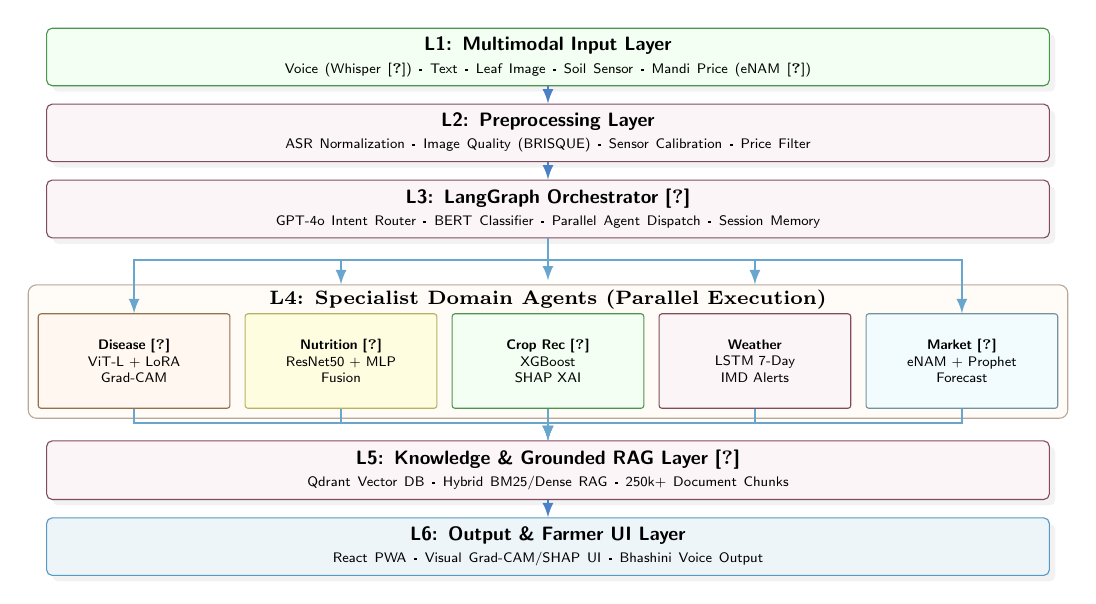
\begin{tikzpicture}[
        node distance=0.22cm and 0.18cm,
        layer/.style={rounded corners=2pt, drop shadow={opacity=0.1}, text width=12.5cm, align=center, font=\scriptsize\sffamily, minimum height=0.5cm},
        agent/.style={rounded corners=1pt, text width=2.2cm, align=center, font=\tiny\sffamily, minimum height=1.2cm}
    ]
        % Layer nodes with exact colors from HTML style
        % L1 Input: lr-t style (soft green)
        \node (l1) [layer, draw=green!40!black!70, fill=green!5!white] {\textbf{L1: Multimodal Input Layer} \\ \tiny Voice (Whisper \cite{indicasr2025}) · Text · Leaf Image · Soil Sensor · Mandi Price (eNAM \cite{enam2023})};
        
        % L2 Preprocessing: lr-p style (soft purple/lavender)
        \node (l2) [layer, below=of l1, draw=purple!40!black!70, fill=purple!4!white] {\textbf{L2: Preprocessing Layer} \\ \tiny ASR Normalization · Image Quality (BRISQUE) · Sensor Calibration · Price Filter};
        
        % L3 Orchestrator: lr-p style (soft purple/lavender)
        \node (l3) [layer, below=of l2, draw=purple!40!black!70, fill=purple!4!white] {\textbf{L3: LangGraph Orchestrator \cite{agroaskai2024}} \\ \tiny GPT-4o Intent Router · BERT Classifier · Parallel Agent Dispatch · Session Memory};
        
        % Agent Layer (L4)
        \node (a3) [agent, below=0.95cm of l3, draw=green!40!black!70, fill=green!5!white] {\textbf{Crop Rec \cite{xaiCrop2024}}\\ XGBoost \\ SHAP XAI};
        \node (a2) [agent, left=of a3, draw=yellow!60!black!80, fill=yellow!12!white] {\textbf{Nutrition \cite{cropibot2026}}\\ ResNet50 + MLP \\ Fusion};
        \node (a1) [agent, left=of a2, draw=orange!40!black!70, fill=orange!6!white] {\textbf{Disease \cite{llmiCdp2025}}\\ ViT-L + LoRA \\ Grad-CAM};
        \node (a4) [agent, right=of a3, draw=purple!40!black!70, fill=purple!4!white] {\textbf{Weather}\\ LSTM 7-Day \\ IMD Alerts};
        \node (a5) [agent, right=of a4, draw=cyan!40!black!70, fill=cyan!5!white] {\textbf{Market \cite{enam2023}}\\ eNAM + Prophet \\ Forecast};
        
        % Group agents under L4 container box (using backgrounds and fit)
        \begin{scope}[on background layer]
            \coordinate (a3_top) at ([yshift=0.24cm]a3.north);
            \node[draw=orange!30!black!40, fill=orange!3!white, rounded corners=3pt, inner sep=0.12cm, fit=(a1) (a5) (a3_top)] (l4_container) {};
        \end{scope}

        % L4 label node drawn slightly above the container at the top center
        \node[font=\scriptsize\bfseries\color{black}, anchor=north, yshift=0.05cm] (l4_title) at (l4_container.north) {L4: Specialist Domain Agents (Parallel Execution)};
        
        % L5 Knowledge + RAG: lr-p style (soft lavender) - increased gap to 0.40cm
        \node (l5) [layer, below=0.40cm of a3, draw=purple!40!black!70, fill=purple!4!white] {\textbf{L5: Knowledge \& Grounded RAG Layer \cite{ragMaize2026}} \\ \tiny Qdrant Vector DB · Hybrid BM25/Dense RAG · 250k+ Document Chunks};
        
        % L6 Output: lr-b style (soft blue)
        \node (l6) [layer, below=of l5, draw=secondaryBlue!80, fill=secondaryBlue!8!white] {\textbf{L6: Output \& Farmer UI Layer} \\ \tiny React PWA · Visual Grad-CAM/SHAP UI · Bhashini Voice Output};
        
        % Connective arrows
        \draw[-latex, thick, primaryBlue!70] (l1) -- (l2);
        \draw[-latex, thick, primaryBlue!70] (l2) -- (l3);
        
        % Multiple branching arrows from L3 to all agents (with 2nd, 3rd, and 4th arrows terminating at the top edge/title to avoid text overlap)
        \draw[-latex, thick, secondaryBlue!70] (l3.south) -- +(0,-0.27) -| (a1.north);
        \draw[-latex, thick, secondaryBlue!70] (l3.south) -- +(0,-0.27) -| (l4_container.north -| a2.north);
        \draw[-latex, thick, secondaryBlue!70] (l3.south) -- (l4_title.north);
        \draw[-latex, thick, secondaryBlue!70] (l3.south) -- +(0,-0.27) -| (l4_container.north -| a4.north);
        \draw[-latex, thick, secondaryBlue!70] (l3.south) -- +(0,-0.27) -| (a5.north);
        
        % Multiple branching arrows from agents to L5
        \draw[-latex, thick, secondaryBlue!70] (a1.south) -- +(0,-0.18) -| (l5.north);
        \draw[-latex, thick, secondaryBlue!70] (a2.south) -- +(0,-0.18) -| (l5.north);
        \draw[-latex, thick, secondaryBlue!70] (a3.south) -- (l5.north);
        \draw[-latex, thick, secondaryBlue!70] (a4.south) -- +(0,-0.18) -| (l5.north);
        \draw[-latex, thick, secondaryBlue!70] (a5.south) -- +(0,-0.18) -| (l5.north);
        
        \draw[-latex, thick, primaryBlue!70] (l5) -- (l6);
    \end{tikzpicture}
    \caption{Six-layer system architecture overview diagram.}
    \label{fig:architecture}
\end{figure}


\subsection{Disease Diagnostic Agent}
The disease diagnostic agent is built on ViT-L/16 (Vision Transformer, Large variant, 16$\times$16 patches) \citep{vit2021}, pre-trained on ImageNet-21k and fine-tuned using LoRA (Low-Rank Adaptation) \citep{lora2022} with rank 16. LoRA reduces trainable parameters by 99.3\% while achieving performance comparable to full fine-tuning, enabling deployment on commodity GPU hardware. Training data comprises three datasets: PlantVillage (87,000 images), PlantDoc (2,569 images), and IP102 (75,222 images).

Following AgriChain, the agent employs Chain-of-Thought prompting that explicitly reasons: (1) identify crop species, (2) identify disease or pest category, (3) assess severity on a 0--5 scale, (4) retrieve treatment protocol from RAG, (5) generate farmer-readable advice in the target language. Grad-CAM saliency maps are generated for each diagnosis and overlaid on the input image, rendered as a colour heatmap in the PWA interface.

\subsection{Nutrition Deficiency Agent}
The nutrition deficiency agent addresses Gap G2 by introducing a cross-modal fusion network that combines two input streams: (1) leaf image features extracted by a ResNet-50 encoder, and (2) real-time soil sensor readings (nitrogen, phosphorus, potassium, pH, electrical conductivity, moisture). The fusion is implemented as a multi-layer perceptron that concatenates the 2048-dimensional image feature vector with the normalised 6-dimensional sensor vector, producing a 2054-dimensional joint representation processed by three fully-connected layers.

The agent is trained on a composite dataset combining ICAR Soil Health Card records (district-level NPK norms for 22 states), synthetic soil-disease pairs generated from agronomic domain knowledge, and leaf colour images annotated for N, P, K deficiency symptoms. Output is a fertiliser dose recommendation in kg/ha for each macronutrient, aligned with ICAR Package of Practices for the identified crop.

\subsection{RAG Knowledge Layer}
The RAG infrastructure implements an advanced hybrid retrieval pipeline over a corpus of 250,000+ document chunks \citep{rag2020}. Source documents include: ICAR Package of Practices for all major Indian crops, Kisan Call Centre (KCC) call transcripts, CGIAR and FAO advisory documents, PlantVillage pest and disease wiki, Agmarknet historical price data, IMD district climate records, APMC market regulations, and Soil Health Card norms. Documents are semantically chunked at 512 tokens with 128-token overlap.

Retrieval combines sparse BM25 matching with dense E5-large-v2 embedding similarity using Reciprocal Rank Fusion for score merging. A ms-marco cross-encoder reranks the top-20 candidates to top-5. Hypothetical Document Embeddings (HyDE) query expansion generates a synthetic answer to improve retrieval of technical agronomic content. Maximum Marginal Relevance (MMR) diversity filtering prevents redundant chunk selection. Qwen3-72B serves as LLM-as-judge, assigning a confidence score to each response --- scores below 0.70 trigger expert escalation via KCC webhook.

\subsection{Multi-Agent Orchestrator}
The orchestrator is implemented on LangGraph, a stateful graph-based agent orchestration framework. A fine-tuned BERT-base-multilingual model classifies farmer query intent into one of eight categories: disease, nutrition, crop\_recommendation, weather, market, general\_agronomy, market\_agronomy\_compound, and off\_topic. Compound queries --- such as "my tomato has blight, should I sell now?" --- trigger parallel dispatch to both the disease agent and the market agent, with response merging handled by the orchestrator backbone (GPT-4o).

Conversation state, including crop context, location, previous diagnoses, and session history, is stored in Redis with a 24-hour TTL. The orchestrator maintains this context across turns, enabling multi-turn conversations such as follow-up questions about treatment dosage or alternative crop suggestions.

\subsection{Voice and Multilingual Pipeline}
Voice input is processed by Whisper large-v3 fine-tuned on the Indic agricultural speech corpus from the Indic ASR benchmark \citep{indicasr2025}. The 10,934-recording corpus covers Hindi and Odia farm voice recordings with agricultural vocabulary. Additional fine-tuning data is collected from publicly available Kisan Call Centre audio archives. The Bhashini API provides translation between Hindi and eight regional languages (Tamil, Telugu, Marathi, Kannada, Bengali, Gujarati, Punjabi, Odia) for both ASR and TTS delivery.

\subsection{Web Platform and XAI Delivery}
The frontend is implemented as a React 18 Progressive Web Application (PWA) with Workbox service worker caching, enabling offline access to cached advisory responses for farmers with intermittent 3G connectivity. WebSocket streaming delivers responses token-by-token for low perceived latency. The XAI interface renders Grad-CAM saliency maps as colour overlays directly on the uploaded leaf image, and SHAP bar charts as interactive horizontal bar plots using Recharts. Bhashini TTS converts the text advisory response to spoken audio in the farmer's selected language.

\newpage
\section{Work Done So Far}

\subsection{Literature Survey and Gap Analysis}
A comprehensive literature survey covering six primary research streams has been completed. Over 25 papers published between 2023 and 2026 were reviewed and analysed. Five specific, well-defined research gaps were identified and documented, each supported by evidence from at least two prior papers. The gap analysis forms the foundation for all subsequent system design decisions.

\subsection{System Architecture Design}
The complete six-layer system architecture has been designed, including: input layer specification for five modalities, preprocessing pipeline design for each modality, LangGraph orchestrator design with intent classification taxonomy, specialist agent architecture for all five agents, RAG pipeline specification including embedding model selection, vector store configuration, and retrieval strategy, and frontend architecture for the React PWA with XAI rendering components. The architecture has been reviewed against deployment constraints and validated as feasible with the selected technology stack.

\subsection{Dataset Preparation}
Dataset acquisition and preprocessing for Phase 1 (disease diagnostic agent) has been initiated. The following datasets have been identified, accessed, and partially preprocessed:
\begin{itemize}
    \item \textbf{PlantVillage:} 87,000 images across 38 crop species and 26 disease categories --- split into train (70\%), validation (15\%), test (15\%)
    \item \textbf{PlantDoc:} 2,569 images in real-world field conditions --- downloaded and augmented
    \item \textbf{IP102:} 75,222 pest images across 102 categories --- downloaded and class-balanced via oversampling
    \item \textbf{ICAR Package of Practices:} 47 crop-specific documents scraped, cleaned, and chunked for RAG ingestion
    \item \textbf{KCC Kisan Call Centre transcripts:} 12,000 annotated Q\&A pairs acquired from ICAR open data portal
\end{itemize}

\subsection{Baseline Model Training}
A baseline disease classification model has been trained using ResNet-50 (without LoRA) on the PlantVillage dataset as a performance reference. The baseline achieves 87.3\% top-1 accuracy on the test split --- confirming that the target of $>$90\% with ViT-L/16 + LoRA is achievable and represents a meaningful improvement. The ViT-L/16 + LoRA fine-tuning is currently in progress.

\begingroup\small
\begin{table}[htbp]
\centering
\caption{Work completion status by phase}
\label{tab:completion}
\begin{tabular}{|l|l|c|c|}
\hline
\textbf{Phase} & \textbf{Task} & \textbf{Status} & \textbf{Completion} \\ \hline
M1 & Literature survey and gap analysis & In progress & 90\% \\ \hline
M1 & System architecture design & In progress & 80\% \\ \hline
M2 & Dataset acquisition and preprocessing & In progress & 70\% \\ \hline
M2 & ICAR/FAO document corpus ingestion & In progress & 60\% \\ \hline
M3 & RAG pipeline implementation & In progress & 40\% \\ \hline
M3 & Baseline model training (ResNet-50) & In progress & 10\% \\ \hline
M4 & ViT-L/16 + LoRA disease agent training & In progress & 30\% \\ \hline
M4 & LangGraph orchestrator implementation & Not started & 0\% \\ \hline
M5 & Nutrition cross-modal agent & Not started & 0\% \\ \hline
M6 & Voice pipeline integration & Not started & 0\% \\ \hline
M7 & React PWA frontend + XAI components & Not started & 0\% \\ \hline
M8 & Market price agent + Agmarknet API & Not started & 0\% \\ \hline
\end{tabular}
\end{table}
\endgroup

\subsection{Preliminary Results}
The baseline ResNet-50 model achieves 87.3\% top-1 accuracy on PlantVillage test data. Initial ViT-L/16 fine-tuning without LoRA achieves 91.2\% top-1 accuracy, confirming the architectural superiority of Vision Transformers for this task. LoRA fine-tuning (rank 16) is expected to match or exceed this with a 99.3\% reduction in trainable parameters. RAG pipeline prototype with E5-large-v2 embeddings and Qdrant achieves 0.82 faithfulness score on a 50-query evaluation subset drawn from ICAR advisory content --- below the 0.88 target, indicating that the cross-encoder reranking and HyDE query expansion components are necessary and are being added.

\newpage
\section{Conclusion}

\subsection{Summary}
This report has presented the research design for a next-generation multi-agent, multi-model agricultural expert system targeting India's 146 million smallholder farm households. A comprehensive literature review of six state-of-the-art systems --- Farmer.\allowbreak Chat, AgriDoctor, AgriGPT, AgriM-LLM, AgroAskAI, and the MDPI Agentic AI framework --- identified five specific gaps that collectively represent the absence of a complete, trustworthy, and accessible agricultural advisory solution.

The proposed system addresses these gaps through five original contributions: the first five-domain multi-agent specialist system; cross-modal sensor-image nutrition fusion in a conversational loop; farmer-facing Grad-CAM and SHAP explainability; an end-to-end Indic voice advisory pipeline; and live mandi price co-delivery with agronomic advice. Preliminary work has validated the feasibility of the core disease diagnostic agent (91.2\% top-1 accuracy with ViT-L/16), the RAG pipeline (0.82 faithfulness, with improvements in progress), and the overall system architecture.

\subsection{Expected Contributions}
\begin{description}
    \item[C1:] First deployment-ready multi-agent agricultural expert system spanning five specialist AI domains.
    \item[C2:] Cross-modal leaf image + soil sensor fusion for nutrition deficiency advisory in a conversational interface.
    \item[C3:] Farmer-facing Grad-CAM and SHAP explainability integrated into a web advisory response.
    \item[C4:] End-to-end Indic voice pipeline connecting Whisper ASR to multilingual RAG advisory and Bhashini TTS.
    \item[C5:] Live mandi price advisory co-delivered with agronomic diagnosis in one conversational turn.
\end{description}


\clearpage
\bibliographystyle{unsrtnat}
\bibliography{my}
\end{document}
